% concatenated from BWX-2025.tex
%  %%%%%%%%%%%%%%%%%%%%%%%%%%%%%%%%%%%%%%%%%%%%%%%%%%%%%%%%%%%%%%%%%%%%%%%%
% \documentclass{amsart}
\documentclass[11pt, reqno]{amsart}
\usepackage{mathrsfs}
\usepackage{amssymb}
\usepackage{amsfonts}
\usepackage{amsmath, color, esvect}
 \usepackage[colorlinks,linkcolor=blue,urlcolor=cyan,citecolor=blue]{hyperref} 
%\usepackage[colorlinks,linkcolor=blue,urlcolor=cyan,citecolor=blue,pagebackref]{hyperref}
\usepackage{genyoungtabtikz}
\usepackage{tikz}
\usepackage{multirow,graphicx}
\usepackage[normalem]{ulem}
\usepackage{multirow}
\usepackage{braket}
\usepackage{cleveref}
\usepackage{caption}
%\usepackage{enumitem}
%\usepackage[T1]{fontenc} 
%\usepackage[utf8]{inputenc} 

%\usepackage[english]{babel}

%\usepackage{biblatex}


%\bibliography{minGK}

% %% show label %%%
% \usepackage{xcolor}
% \usepackage[color]{showkeys}
% \definecolor{refkey}{gray}{.45}
% \definecolor{labelkey}{gray}{.45}
% \definecolor{citekey}{gray}{.45}











% \usepackage[backend=biber,style=alphabetic,sorting=nyt]{biblatex}
% \addbibresource{minGK.bib}

%\newcommand\reduline{\bgroup\markoverwith
%     {\textcolor{red}{\rule[0.5ex]{2pt}{1pt}}}\ULon}

%\DeclareUnicodeCharacter{0306}{}

%\usepackage{times}

\makeatletter
\def\inn#1#2{\left\langle 
      \def\ta{#1}\def\tb{#2}
      \ifx\ta\@empty{\;} \else {\ta}\fi ,
      \ifx\tb\@empty{\;} \else {\tb}\fi
      \right\rangle} 
\makeatother


\def\fhh{\mathfrak{h}}
\def\fbb{\mathfrak{b}}
\def\fnn{\mathfrak{n}}
\def\fpp{\mathfrak{p}}
\def\fqq{\mathfrak{q}}
\def\fuu{\mathfrak{u}}
\def\fll{\mathfrak{l}}
\def\fbb{\mathfrak{b}}
\def\fgg{\mathfrak{g}}
\def\fkk{\mathfrak{k}}
\def\cC{\mathcal{C}}
\def\cD{\mathcal{D}}
\def\cO{\mathcal{O}}
\def\cV{\mathcal{V}}
\def\cQ{\mathcal{Q}}
\def\cM{\mathcal{M}}
\def\cL{\mathcal{L}}
\def\cU{\mathcal{U}}
\def\tM{\tilde{M}}
\def\CC{\mathrm{CC}}
\def\Gr{\mathrm{Gr}}
\def\gr{\mathrm{gr}}
\def\bR{\mathbb{R}}
\def\fD{\mathfrak{D}}
\def\mystrut{\vbox to .15in{}}

\newcommand{\mb}{\mathbf}
\newcommand{\bb}{\mathbb}
\newcommand{\ms}{\mathscr}
\newcommand{\mr}{\mathrm}
\newcommand{\frk}{\mathfrak}
\newcommand{\Ree}{\mathrm{Re}}

\newcommand{\Wsmall}{W_{[\lambda]}}

\newcommand{\psp}{\vspace{0.4cm}}
\newcommand{\pse}{\vspace{0.2cm}}
\newcommand{\ptl}{\partial}
\newcommand{\dlt}{\delta}
\newcommand{\sgm}{\sigma}
\newcommand{\al}{\alpha}
\newcommand{\be}{\beta}
%\newcommand{\G}{\Gamma}
\newcommand{\g}{\gamma}
\newcommand{\gm}{\gamma}
\newcommand{\vs}{\varsigma}
\newcommand{\Lmd}{\Lambda}
\newcommand{\lmd}{\lambda}
\newcommand{\td}{\tilde}
\newcommand{\vf}{\varphi}
\newcommand{\yt}{Y^{\nu}}
\newcommand{\wt}{\mbox{wt}\:}
\newcommand{\der}{\mbox{Der}\:}
\newcommand{\es}{\epsilon}
\newcommand{\dmd}{\diamond}
\newcommand{\clt}{\clubsuit}
\newcommand{\vt}{\vartheta}
\newcommand{\ves}{\varepsilon}
\newcommand{\dg}{\dagger}
\newcommand{\rf}[1]{#1\bar{~}}
\newcommand{\lam}{\lambda}
\newcommand{\rcell}{\sim_R}

\newcommand{\ep}{\varepsilon}


\newcommand{\fra}{\mathfrak{a}}
\newcommand{\frb}{\mathfrak{b}}
\newcommand{\fre}{\mathfrak{e}}
\newcommand{\frf}{\mathfrak{f}}
\newcommand{\frg}{\mathfrak{g}}
\newcommand{\frh}{\mathfrak{h}}
\newcommand{\frkk}{\mathfrak{k}}
\newcommand{\frl}{\mathfrak{l}}
\newcommand{\frm}{\mathfrak{m}}
\newcommand{\frn}{\mathfrak{n}}
\newcommand{\fro}{\mathfrak{o}}
\newcommand{\frp}{\mathfrak{p}}
\newcommand{\frq}{\mathfrak{q}}
\newcommand{\frr}{\mathfrak{r}}
\newcommand{\frs}{\mathfrak{s}}
\newcommand{\frt}{\mathfrak{t}}
\newcommand{\fru}{\mathfrak{u}}
\newcommand{\frv}{\mathfrak{v}}
\newcommand{\frgl}{\mathfrak{gl}}
\newcommand{\frsl}{\mathfrak{sl}}
\newcommand{\frsu}{\mathfrak{su}}
\newcommand{\frso}{\mathfrak{so}}
\newcommand{\frsp}{\mathfrak{sp}}

\newcommand{\caA}{\mathcal{A}}
\newcommand{\caB}{\mathcal{B}}
\newcommand{\caC}{\mathcal{C}}
\newcommand{\caD}{\mathcal{D}}
\newcommand{\caE}{\mathcal{E}}
\newcommand{\caF}{\mathcal{F}}
\newcommand{\caG}{\mathcal{G}}
\newcommand{\caH}{\mathcal{H}}
\newcommand{\caI}{\mathcal{I}}
\newcommand{\caJ}{\mathcal{J}}
\newcommand{\caK}{\mathcal{K}}
\newcommand{\caL}{\mathcal{L}}
\newcommand{\caM}{\mathcal{M}}
\newcommand{\caN}{\mathcal{N}}
\newcommand{\caO}{\mathcal{O}}
\newcommand{\caP}{\mathcal{P}}
\newcommand{\caQ}{\mathcal{Q}}
\newcommand{\caR}{\mathcal{R}}
\newcommand{\caS}{\mathcal{S}}
\newcommand{\caT}{\mathcal{T}}
\newcommand{\caU}{\mathcal{U}}
\newcommand{\caV}{\mathcal{V}}
\newcommand{\caW}{\mathcal{W}}
\newcommand{\caX}{\mathcal{X}}
\newcommand{\caY}{\mathcal{Y}}
\newcommand{\caZ}{\mathcal{Z}}
\newcommand{\hobox}[3]{\draw (0+#1,0-#2) rectangle (1+#1,-1-#2)++(-0.5,+0.5) node {$ #3$};}

\newcommand{\gk}{Gelfand--Kirillov dimension }
\newcommand{\gks}{Gelfand--Kirillov dimensions }
\newcommand{\aff}{\mathbf{a}}
\newcommand{\mc}[1]{\mathcal{#1}}
\newcommand{\msc}[1]{\mathscr{#1}}
\newcommand{\mf}[1]{\mathfrak{#1}}
\renewcommand{\subset}{\subseteq}
\newcommand{\rar}{\rightarrow}
\newcommand{\bil}[2]{\langle{#1},{#2}^{\vee} \rangle }
\newcommand{\hs}{ \mathfrak{h}^*}
\newcommand{\Ocat}{\mathscr{O}}

\newcommand{\Ann}{\operatorname{Ann}}
\newcommand{\gkd}{\operatorname{GKdim}}
\renewcommand{\hom}{\operatorname{Hom}}
\newcommand{\sln}{\mathfrak{sl}(n)}
\newcommand{\lambdarho}{\lambda+\rho=(\lambda_1,\lambda_2,\cdots,\lambda_n)}
\newcommand{\sn}{\mf{S}_n}
\newcommand{\su}{{SU}}
\newcommand{\nodd}{}

\newcommand{\sh}{\operatorname{sh}}
\newcommand{\ev}{^{\mathrm{ev}}}
\newcommand{\od}{^{\mathrm{odd}}}

\newcommand{\gln}{\mathfrak{gl}(n,\mathbb{C})}

\newcommand{\spn}{\mathfrak{sp}(n,\mathbb{C})}

\newcommand{\sob}{\mathfrak{so}(2n+1,\mathbb{C})}

\newcommand{\sod}{\mathfrak{so}(2n,\mathbb{C})}

\newtheorem{Thm}{Theorem}[section]
\newtheorem{cor}[Thm]{Corollary}
\newtheorem{prop}[Thm]{Proposition}
\newtheorem{lem}[Thm]{Lemma}

\newtheorem{remarks}[Thm]{Remarks}
\newtheorem{question}[Thm]{Question}

\theoremstyle{definition}
\newtheorem{Rem}[Thm]{Remark}
\newtheorem{dfn}[Thm]{Definition}
\newtheorem{notation}[Thm]{Notation}
\newtheorem{example}[Thm]{Example}
\newtheorem{Con}[Thm]{Conjecture}

\newtheorem{thmA}{Theorem}
\renewcommand*{\thethmA}{\Alph{thmA}}

\numberwithin{equation}{section} 

\newcommand{\rmk}[2]{\textcolor{red}{#1}
\marginpar{
\color{red}\footnotesize#2
}}

\newcommand{\cOmin}{\cO_{\mathrm{min}}}

\setlength{\abovecaptionskip}{5pt}
\setlength{\belowcaptionskip}{5pt}

%\def\showtrivial{}

\newcommand{\trivial}[2][]{\if\relax\detokenize{#1}\relax{\color{red}\vspace{0em} $[$  #2 $]$}\else
\ifx#1h
\ifcsname showtrivial\endcsname{\color{orange} \vspace{0em}  $[$ #2 $]$}\fi\else{\colorWrong argument!}\fi\fi\ignorespaces}



\usepackage{enumitem}
\setlist[enumerate,1]{font=\textup,
	leftmargin=5mm,labelsep=0.2em,topsep=1mm,itemsep=1mm,itemindent=1em,listparindent=1em}
\setlist[enumerate,2]{font=\textup, leftmargin=3mm,labelsep=0.2mm,topsep=1mm,itemsep=1mm,itemindent=1em}
\setlist[enumerate,3]{font=\textup, leftmargin=4mm,labelsep=1mm,topsep=1mm,itemsep=1mm,itemindent=1em,listparindent=1em}
\setlist[enumerate,4]{font=\textup, leftmargin=5mm,labelsep=1mm,topsep=1mm,itemsep=1mm,itemindent=1em,listparindent=1em}




\newcommand{\fa}{\mathfrak{a}}
\newcommand{\fb}{\mathfrak{b}}
%\newcommand{\fre}{\mathfrak{e}}
%\newcommand{\frf}{\mathfrak{f}}
\newcommand{\fg}{\mathfrak{g}}
\newcommand{\fh}{\mathfrak{h}}
\newcommand{\fk}{\mathfrak{k}}
\newcommand{\fl}{\mathfrak{l}}
\newcommand{\fm}{\mathfrak{m}}
%\newcommand{\frn}{\mathfrak{n}}
%\newcommand{\fro}{\mathfrak{o}}
\newcommand{\fp}{\mathfrak{p}}
\newcommand{\fq}{\mathfrak{q}}
%\newcommand{\frr}{\mathfrak{r}}
%\newcommand{\frs}{\mathfrak{s}}

\newcommand{\fu}{\mathfrak{u}}
%\newcommand{\frv}{\mathfrak{v}}
%\newcommand{\frgl}{\mathfrak{gl}}
%\newcommand{\frsl}{\mathfrak{sl}}
%\newcommand{\frsu}{\mathfrak{su}}
%\newcommand{\frso}{\mathfrak{so}}
%\newcommand{\frsp}{\mathfrak{sp}}
%\newcommand{\gkd}{\operatorname{GKdim}}
\newcommand{\bbC}{\mathbb{C}}
\newcommand{\bbD}{\mathbb{D}}
\newcommand{\bbH}{\mathbb{H}}
\newcommand{\bbN}{\mathbb{N}}
\newcommand{\bbQ}{\mathbb{Q}}
\newcommand{\RR}{\mathbb{R}}
\newcommand{\bbT}{\mathbb{T}}
\newcommand{\bbZ}{\mathbb{Z}}

% %
 \begin{document}
\title[Minimal highest weight modules]{Associated varieties of integral 
minimal  highest weight modules}
% \title[Smooth right cells]{A characterization of Kazhdan--Lusztig right cells containing smooth elements }

\author{Zhanqiang Bai}
\address[Bai]{School of Mathematical Sciences, Soochow University, Suzhou 215006, P. R. China}
\email{zqbai@suda.edu.cn}

\author{Jing Jiang*}
\thanks{* Corresponding author}
\address[Jiang]{
School of Mathematical Sciences, East China Normal University, Shanghai 200241, China} 
\email{jjsd6514@163.com}


\author{Rui Wang}
\address[Wang]{School of Mathematical Sciences, Soochow University, Suzhou 215006, P. R. China}
\email{19962879291@163.com}

% \author{Xun Xie}
% \address[Xie]{School of Mathematics and Statistics, Beijing Institute of Technology, Beijing 100081, China}
% \email{xieg7@163.com}


\subjclass[2010]{Primary 22E47, 17B10; Secondary 05E10}


\bigskip

\begin{abstract}
Let $\mathfrak{g}$ be a complex simple Lie algebra and $L(\lambda)$ be a highest weight  module of $\mathfrak{g}$ with highest weight $\lambda-\rho$, where $\rho$ is half the sum of positive roots.    A simple  $\fgg$-module $L_w:=L(-w\rho)$ is called 
 integral minimal if the associated variety of its annihilator ideal equals the closure of the minimal special nilpotent orbit. 
  In this paper, we  find that the  associated variety of  any integral minimal module $L_w$ is irreducible and equal to the orbital variety corresponding to the minimal length element in the Kazhdan--Lusztig right cell containing $w$. 





\noindent{\textbf{Keywords:} Highest weight module; associated variety;
nilpotent orbit;  Schubert variety;  Kazhdan--Lusztig  cell.}
\end{abstract}
% Schubert variety; Pattern avoidance; Knuth relation;

\maketitle

	%\setcounter{tocdepth}{1}
	\tableofcontents
\section{ Introduction}

Let $G$ be a simple Lie Group. Let $\mathfrak{g}$ be its simple complex Lie algebra and $\mathfrak{h}$ be a Cartan subalgebra.
For any finitely generated $U(\mathfrak{g})$-module $M$, Bernstein \cite{Be} defined the associated variety $V(M)$ in the dual space $\mathfrak{g}^{\ast}$, whose dimension coincides with the Gelfand–Kirillov (GK) dimension of $M$ \cite{Vo78}. This variety is a useful invariant in the study of $U(\mathfrak{g})$-modules, especially for highest weight modules, see for example \cite{BoB3, Ta, Mel93, Mc00, Wi}. But in general, computing this invariant for an irreducible module is a highly nontrivial problem.




Let $\Phi^+\subset\Phi$ be the set of positive roots determined by a Borel subalgebra $\mathfrak{b}$ of $\mathfrak{g}$. Denote by $\Pi$ the set of simple roots in $\Phi^+$. Fix a Borel subgroup $B\subset G$ corresponding to $\mathfrak{b}$. We have  a triangular decomposition $\mathfrak{g}=\mathfrak{n}\oplus \mathfrak{h} \oplus \mathfrak{n}^-$. Choose a subset ${\rm J}\subset \Pi$. Then it generates a subsystem
$\Phi_{\rm J}\subset\Phi$.
Let $\fp_{\rm J}$ be the standard parabolic subalgebra corresponding to ${\rm J}$ with Levi decomposition $\fp_{\rm J}=\fl_{\rm J}\oplus\fu_{\rm J}$.
% Fix a parabolic subgroup $ P=P_{\rm J} $ such that $B\subset P_{\rm J}\subset G$ and $\text{Lie}(P_{\rm J})=\mathfrak{p}_{\rm J}$.
For a \(\Phi^{+}(\mathfrak{l}_{\rm J})\)-dominant integral weight \(\lambda \in \mathfrak{h}^{*}\), let \(F(\lambda)\) be the irreducible \(\mathfrak{l}_{\rm J}\)-module with highest weight \(\lambda-\rho\), 
 where $\rho$ is half the sum of positive roots. Viewing \(F(\lambda)\) as a \(\mathfrak{p}_{\rm J} = \mathfrak{l}_{\rm J} \oplus \mathfrak{u}_{\rm J}^{+}\)-module (with the nilradical acting trivially), we define the generalized Verma module by
\[
N_{\rm J}(\lambda) := U(\mathfrak{g}) \otimes_{U(\mathfrak{p}_{\rm J})} F(\lambda).
\]
Let \(L(\lambda)\) denote the irreducible quotient of \(N_{\rm J}(\lambda)\), which is a highest weight module of $\mathfrak{g}$ with highest
weight \(\lambda-\rho\).





 %  We use $L_w$ to denote the simple highest weight $\mathfrak{g}$-module of highest weight $-w\rho-\rho$ with  $w\in W$. 
 % Joseph \cite{Jo84} proved that the associated variety $V(L_w)$ is a union of orbital varieties defined as follows. Let $\mathcal{O}\subseteq \mathfrak{g}$ be a nilpotent $G$-orbit. The irreducible components of $\overline{\mathcal{O}}\cap \mathfrak{n}$ are called {\it orbital varieties} of  $\mathcal{O}$. They all take the form $\mathcal{V}(w)=\overline{B(\mathfrak{n}\cap w\mathfrak{n})}$ for some $w\in W$.  The associated variety  $V(L_w)$ is  called {\it irreducible}  if it contains only one orbital variety. When $L(\lambda)$ is a highest weight Harish-Chandra module, the associated variety $V(L(\lambda))$ was characterized in Bai--Xiao--Xie \cite{BXX} and Bai--Hunziker--Xie--Zierau \cite{BHXZ}. When $L(\lambda)$ has the minimal Gelfand--Kirillov dimension, the associated variety $V(L(\lambda))$ was characterized in Bai--Ma--Xiao--Xie \cite{BMXX}.
 % The structure of $V(L_w)$ or $V(L(\lambda)) $ is  unknown in general, see for example \cite{Ta,Wi,BoB3}. 

Denote
by $W$ the Weyl group of $\Phi$. Let $L_w$ denote the simple highest weight $\mathfrak{g}$-module with highest weight $-w\rho-\rho$, where $w\in W$.  
Joseph \cite{Jo84} found that the associated variety $V(L_w)$ is a union of orbital varieties, which are defined as follows. For a nilpotent $G$-orbit $\mathcal{O}\subseteq \mathfrak{g}$, the irreducible components of $\overline{\mathcal{O}}\cap \mathfrak{n}$ are called the {\it orbital varieties} of $\mathcal{O}$. Each such component can be expressed as $\mathcal{V}(w)=\overline{B(\mathfrak{n}\cap w\mathfrak{n})}$ for some $w\in W$. The associated variety $V(L_w)$ is said to be {\it irreducible} if it consists of a single orbital variety. For highest weight Harish-Chandra modules $L(\lambda)$, the associated variety $V(L(\lambda))$ has been characterized in Bai--Xiao--Xie \cite{BXX} and Bai--Hunziker--Xie--Zierau \cite{BHXZ}.  In general, however, the structure of $V(L_w)$ or $V(L(\lambda))$ remains unknown; see, for example, \cite{BoB3,Ta,Wi}. 

% Moreover, when $L(\lambda)$ has minimal Gelfand--Kirillov dimension (equivalently, the associated variety of the annihilator ideal ${\Ann(L(\lambda))}$ is just the closure of the minimal nilpotent orbit $\mathcal{O}_{\rm m}$), the associated variety  $V(L(\lambda))$ was described in Bai--Ma--Xiao--Xie \cite{BMXX}.

As noted in \cite{BoB3}, the associated variety $V(L_w)$ is intimately connected to Schubert varieties. In the following, we recall some of these relations.

 The  flag variety $G/B$ decomposes into a disjoint union of Schubert
cells $BwB/B$, where $w$  is an element in the  corresponding Weyl group $W$. The Schubert
varieties $X(w)=\overline{BwB/B}$ are the closures of the Schubert cells.
Schubert varieties are fundamental objects in algebraic geometry, representation theory, and combinatorics.  $X(w)$ is said to be  smooth if it is a smooth algebraic variety at every point, and  rationally smooth if the Poincar\'{e} polynomial $p_w(t)=\sum_{v\leq w}t^{\ell(v)}$is palindromic, where $\leq$ is the Bruhat order on $W$ and ${\ell}(v)$  the length of $v$.  


% The study of  smoothness and rational smoothness of Schubert varieties has been a central theme since the foundational work of Lakshmibai and Sandhya \cite{LS-90}, who gave a combinatorial criterion for smoothness in type \(A\): a Schubert variety \(X(w) \subset SL(n)/B\) is smooth if and only if the permutation \(w\in S_n\) avoids the patterns $3412$ and $4231$. This result was later extended to smoothness and rational smoothness for other classical types by Billey \cite{Bi-98}. Billey and Postnikov \cite{BP-05} introduced a uniform approach using root subsystems and embeddings. They showed that, for any semisimple \(G\), the (rational) smoothness of \(X(w) \subset G/B\) can be detected by avoiding a finite list of patterns arising from stellar root subsystems (e.g., \(B_2,G_2,A_3, B_3,C_3, D_4\)). 
Investigations into the smoothness and rational smoothness of Schubert varieties have been a major focus since the seminal work of Lakshmibai and Sandhya \cite{LS-90}, who provided a combinatorial characterization for smoothness in type \(A\): a Schubert variety \(X(w) \subset SL(n)/B\) is smooth precisely when the permutation \(w\in S_n\) avoids the patterns $3412$ and $4231$. This result was subsequently generalized to smoothness and rational smoothness in other classical types by Billey \cite{Bi-98}. Then Billey and Postnikov \cite{BP-05} developed a unified method based on root subsystems and embeddings. They demonstrated that, for any semisimple \(G\), the (rational) smoothness of \(X(w) \subset G/B\) is determined by pattern avoidance with respect to a finite list of patterns originating from stellar root subsystems (e.g., \(B_2,G_2,A_3, B_3,C_3, D_4\)). From now on, the corresponding Weyl group  element $w$ for a smooth Schubert variety $X(w)$ is called a smooth element. 


We refer to \cite{KL79} or \S \ref{KL-cells} for the definition of Kazhdan--Lusztig right (resp. left and two-sided)  cell equivalence relation and use ${\sim}_R$ (resp. ${\sim}_L$ and ${\sim}_{LR}$)  to denote the right  (resp. left and two-sided) cell equivalence relation. We use $\mathcal{C}_R(w)$ (resp. $\mathcal{C}_L(w)$ and $\mathcal{C}_{LR}(w)$) to denote a KL right (resp. left and two-sided) cell  which contains $w$.

 

From \cite{Jo84}, we know that  the associated variety $V (L_w)$ is constant on each KL right cell.
It is also known that  the associated variety $V (L_w)=\mathcal{V}(w)$ if the Schubert variety $X(w)$ is smooth, see for example \cite[Cor. 4.3.2]{BoB3}.
Therefore, the associated variety $V (L_w)$ will be irreducible if the KL right  cell contains a smooth element. For type $A$, Bai and Chen \cite{Bchen} had given an efficient algorithm to find out all the smooth
elements in a given KL right cell.

Let $\mathcal{C}$ be the two-sided cell of $W$  consisting of elements which have a  a unique reduced expression.
In this paper, first we characterize  the smooth Schubert varieties in a given KL right cell of $w_0\mathcal{C}$, where $w_0$ is the longest element of the Weyl group $W$. 

\begin{Thm}\label{smcell}
    Let $\mathcal{C}_i$ be the KL  right cell containing the simple reflection $s_i=s_{\alpha_i}$. Then the smooth elements $S(w_0\mathcal{C}_i)$ of  the KL right cell $w_0\mathcal{C}_i$ are given as follows:
    \begin{enumerate}
        \item For type $A_{n}$, we have
$S(w_0\mathcal{C}_{1})=w_0\mathcal{C}_{1}$, $S(w_0\mathcal{C}_{n})=w_0\mathcal{C}_{n}$ and   $$S(w_0\mathcal{C}_{i})=\{w_0s_is_{i-1}\cdots s_{1},w_0s_is_{i+1}\cdots s_{n}\} \text{~for~} 2\leq i\leq n-1.$$
        \item For type $B_n$, we have $$S(w_0\mathcal{C}_1)=\{w_0s_1\cdots s_ns_{n-1}\cdots s_{n-j+1}\mid 1\leq j\leq n\},$$ $$S(w_0\mathcal{C}_n)=\{w_0s_ns_{n-1}\cdots s_1\}$$ and 
    $$S(w_0\mathcal{C}_i)=\{w_0s_is_{i+1}\cdots s_ns_{n-1}\cdots s_1\}\text{~for~}2\leq i\leq n-1.$$
        \item For type $C_n$, we have $S(w_0\mathcal{C}_1)=w_0\mathcal{C}_1$, $$S(w_0\mathcal{C}_n)=\{w_0s_ns_{n-1}\cdots s_1\}$$ and
    $$S(w_0\mathcal{C}_i)=\{w_0s_is_{i-1}\cdots s_1, w_0s_is_{i+1}\cdots s_ns_{n-1}\cdots s_{1}\}\text{~for~}2\leq i\leq n-1.$$
        \item  For type $D_n$ with $n\geq 4$, we have  
$$S(w_0\mathcal{C}_1)=\{w_0s_1\cdots s_{n-2}s_{n-1},\; w_0s_1\cdots s_{n-2}s_{n}\}$$ 
and $$S(w_0\mathcal{C}_{i})=\varnothing\text{~for~} 2\leq i\leq n-2.$$
For $n=4$, we have $$S(w_0\mathcal{C}_{3})=\{w_0s_{3}s_{2}s_1,w_0s_{3}s_{2}s_4\}$$ and  $$S(w_0\mathcal{C}_4)=\{w_0s_{4}s_{2} s_1,w_0s_{4}s_{2} s_3\}.$$
Moreover, for $n\geq 5$, we have $$S(w_0\mathcal{C}_{n-1})=\{w_0s_{n-1}s_{n-2}\cdots s_1\},$$ $$S(w_0\mathcal{C}_n)=\{w_0s_{n}s_{n-2}\cdots s_1\}.$$ 
        \item For type $E_r$ with $r=6,7,8$, we have
$$S(w_0\mathcal{C}_{i})=\varnothing\text{~for~} 1\leq i\leq r.$$
        \item For type $F_4$, we have $$S(w_0\mathcal{C}_{i})=\varnothing\text{~for~} 1\leq i\leq 4.$$
        \item For type $G_2$, we have 
$$S(w_0\mathcal{C}_{1})=\{s_{2},s_{2}s_1, s_2s_1s_2\}$$ and 
$$S(w_0\mathcal{C}_{2})=\{s_{1},s_{1}s_2\}.$$     
    \end{enumerate}
\end{Thm}

To determine the smoothness of $X(w)$ for $w\in w_0\mathcal{C}$, we have implemented an algorithm in Python, available at
\begin{center}
\url{https://github.com/JingJiang-web/smooth-Schubert-variety}.
\end{center}

% For type $E$ and $F_4$, the algorithm is based on the following steps.
% \begin{enumerate}
%     \item For $w\in W$, we can compute the inversion set $\Phi_w=\Phi^+\cap w (\Phi^-)$ by \cite[§5.6-Exer.~1]{hum90}.

%     \item For type $E$ (resp. $F$), identify all root subsystems $\Delta$ of type $A_3$, $D_4$ (resp. $B_2$, $A_3$, $B_3$, $C_3$) by \cite[Lem. 3.5]{BGWX}.

%     \item Since the elements of $\Phi_w$ are positive roots, then $\Delta_\sigma=\Phi_w\cap \Delta=\Phi_w\cap\Delta^+$ is the inversion set for a unique $\sigma\in W(\Delta)$ in the Weyl group of $\Delta$, where $\Delta^+=\Delta\cap\Phi^+$ is the positive root system of $\Delta$.

%     \item Given the inversion set $\Delta_\sigma$, we obtain $\sigma$ by  \cite[§5.6-Exer.~1]{hum90}:
%     Denote $\Delta_\sigma=\{\gamma_1,\gamma_2,\cdots,\gamma_k\}$, if $\gamma_{i_1}$ is a simple root of $\Delta$, let $$I_1=s_{\gamma_{i_1}}(\Delta_\sigma\setminus\{\gamma_{i_1}\})=\Delta_{s_{\gamma_{i_1}}\sigma}.$$
% If there is a simple root $\gamma_{i_1}\in I_1$ of $\Delta$, let $$I_2=s_{\gamma_{i_2}}(I_1\setminus\{\gamma_{i_2}\})=\Delta_{s_{\gamma_{i_2}}s_{\gamma_{i_1}}\sigma}.$$
% Repeat the above steps, we can get that $$I_k=s_{\gamma_{i_k}}(I_{k-1}\setminus\{\gamma_{i_k}\})=\Delta_{s_{\gamma_{i_k}}\cdots s_{\gamma_{i_2}}s_{\gamma_{i_1}}\sigma}=\varnothing.$$
% Then $\sigma=s_{\gamma_{i_1}}s_{\gamma_{i_2}}\cdots s_{\gamma_{i_k}}$.

%     \item If $\sigma$ avoids all patterns listed in Theorem \ref{BP-patterns} for all root subsystems, then $X(w)$ is smooth. Otherwise, $X(w)$ is non-smooth.
% \end{enumerate}

For a highest weight $\mathfrak{g}$-module $L(\lambda)$, the annihilator $\mathrm{Ann}(L(\lambda))$ is a primitive ideal in the enveloping algebra $U(\mathfrak{g})$. The associated graded ideal $\mathrm{gr}(\mathrm{Ann}(L(\lambda)))$ is an ideal inside the symmetric algebra $S(\mathfrak{g})$, which is naturally isomorphic to $\mathrm{gr}(U(\mathfrak{g}))$. The associated variety of  the quotient module $U(\mathfrak{g})/\mathrm{Ann}(L(\lambda))$ is defined as the zero locus of $\mathrm{gr}(\mathrm{Ann}(L(\lambda)))$ in $\mathfrak{g}^*$; this set is called the {\it annihilator variety} of $L(\lambda)$ and is known to be the Zariski closure of a nilpotent orbit $\mathcal{O}_{\mathrm{Ann}(L(\lambda))}$ in $\mathfrak{g}^*$ \cite{Jo85}.  In \cite{BMW} and \cite{BGWX}, the annihilator variety of a highest weight module had been given in a simple way by using the  Robinson--Schensted algorithm and Sommers duality.
But the associated variety of a highest weight module is still a challenging problem. 

In the case where $\mathcal{O}_{\mathrm{Ann}(L(\lambda))}$ coincides with $\mathcal{O}_{\min}$, the unique minimal nilpotent orbit of $\mathfrak{g}^*$, the associated variety $V(L(\lambda))$ had been given in a simple and uniform characterization by Bai--Ma--Xiao--Xie \cite{BMXX}. From  \cite{BMXX}, we know that there exists a unique minimal special nilpotent orbit (see \cite[\S 6.3]{CM} for the definition of special orbit), denoted $\mathcal{O}_{\mathrm{ms}}$. It satisfies $\mathcal{O}_{\mathrm{ms}} = \mathcal{O}_{\min}$ for simply laced Lie algebras, whereas $\mathcal{O}_{\mathrm{ms}} \neq \mathcal{O}_{\min}$ in the non-simply laced cases. It is known that the minimal special orbit $\mathcal{O}_{{\rm ms}}$ corresponds to the two-sided cell $w_0\mathcal{C}$, see for example \cite{BV82,BMXX,BGWX}. From Kobayashi \cite{Ko11}, we know that small representations of a group will reflect large symmetries in a representation space. This is our motivation for studying small representations of Lie algebras and Lie groups.

% For a highest weight $\mathfrak{g}$-module $L(\lambda)$,  its annihilator $\mathrm{Ann}(L(\lambda))$ is a primitive ideal of $U(\mathfrak{g})$. The associated graded ideal $\mathrm{gr}(\mathrm{Ann}(M))$ is an ideal of the symmetric algebra $S(\mathfrak{g}) \simeq \mathrm{gr}(U(\mathfrak{g}))$. The associated variety  of the quotient module $U(\mathfrak{g})/\mathrm{Ann}(L(\lambda))$ is the zero set of $\mathrm{gr}(\mathrm{Ann}(L(\lambda)))$ in $\mathfrak{g}^*$. It  is called the annihilator variety of $L(\lambda)$, which is known to be the closure of a nilpotent orbit $\mathcal{O}_{{\rm Ann}(L(\lambda))}$ in $\mathfrak{g}^*$ \cite{Jo85}. 


% When $\mathcal{O}_{{\rm Ann}(L(\lambda))}=\mathcal{O}_{\min}$ where $\mathcal{O}_{\min}$ is the unique minimal nilpotent orbit of $\mathfrak{g}^*$,  the associated variety $V(L(\lambda))$ had been given in a simple uniform way by Bai--Ma--Xiao--Xie \cite{BMXX}. From \cite{BMXX}, we know that there is a minimal special nilpotent orbit $\mathcal{O}_{\rm ms}$. We have $\mathcal{O}_{\rm ms}=\mathcal{O}_{\rm mim}$ for the simply laced cases and $\mathcal{O}_{\rm ms}\neq\mathcal{O}_{\rm mim}$ for non-simply laced cases.

% It is natural to expect a more explicit description of the associated variety for simple $U(\mathfrak{g})$-modules $L$ whose associated orbit $\mathcal{O}_L$ coincides with the minimal nilpotent coadjoint orbit $\mathcal{O}_{\min}$ of $\mathfrak{g}^*$. Such an $L$ is called \textit{minimal}. Let $\mathcal{J} = \mathrm{Ann}(L)$. Minimality of $L$ implies that the radical $\sqrt{\mathrm{gr}\,\mathcal{J}}$ of the graded ideal $\mathrm{gr}\,\mathcal{J}$ equals the ideal $\mathcal{I}(\mathcal{O}_{\min})$ of functions vanishing on $\mathcal{O}_{\min}$.





% In \cite{BMXX}, the associated variety $V(L(\lambda))$ had been given in a simple uniform way when $L(\lambda)$ is a minimal highest weight module. For non-simply laced types, the minimal Gelfand--Kirillov dimension of $L_w$ for all $w\in W$ is different from
 

By using properties of the associated varieties of highest weight modules and Theorem \ref{smcell}, we can obtain the following result.




\begin{Thm}\label{AV-min}
% Suppose that $L_w$ has the  minimal
% Gelfand--Kirillov dimension for all $w\in W$.
Suppose that we have $\mathcal{O}_{{\rm Ann}(L_w)}=\mathcal{O}_{{\rm ms}}$.
Then the associated variety $V(L_w)$ is irreducible and can be given as follows:
\begin{enumerate}
   \item For non-simply laced types,  we have $V(L_w)=\mathcal{V}(w_{\rm min})$ when $w\in w_0\mathcal{C}_i$, where $w_{\rm min}$ denotes the unique minimal length element in the KL right cell $w_0\mathcal{C}_i$.
   
 \item For simply laced types, we have $V(L_w)=\mathcal{V}(w_{\rm max})=\mathcal{V}(w_{\rm min})$ when $w\in w_0\mathcal{C}_i$, where $w_{\rm max}=w_0s_i$ is the unique maximal length  element  in the KL right cell $w_0\mathcal{C}_i$.
  
\end{enumerate}

% Let $G/P_{\rm J}$ be cominuscule.
%    Suppose $v\in W^{\rm J}$. The Schubert variety $X_{P_J}(v) \subset G/P_{\rm J}$ is smooth if and only if the Schubert variety $X({vw_{\rm J}}) \subset G/B$ is smooth, where $w_{\rm J}$ is the longest element in the parabolic subgroup $W_{\rm J}$.
\end{Thm}





  This paper is organized as follows. In \S \ref{pre}, we  give some necessary preliminaries about the Schubert varieties, associated varieties of highest weight modules and Kazhdan--Lusztig cells. In \S \ref{section-A}, \S \ref{typebc}, \S \ref{typed}, \S \ref{typeef} and \S \ref{typeg2}, we characterize the smooth elements  in the KL right cell $w_0\mathcal{C}_i$ and  the associated variety of $L_w$ in the case of type $A_{n}$, $B_n$ and $C_n$, $D_n$, $E$ and $F_4$, and $G_2$ respectively.

 



\section{Preliminaries}\label{pre}
In this section, we give some brief preliminaries on Schubert varieties, associated varieties of highest weight modules and Kazhdan--Lusztig cells.


% Let $\fg$   be a complex simple Lie algebra of rank $n$. We fix a Cartan subalgebra $\fh$ of $\fg$, and denote 
% by $\Phi\subset \fh^*$ the root system of $\fg$ with respect to $\fh$.
% We choose a simple system  $\Pi\subset \Phi$ and write $\Pi=\{\alpha_1,\ldots,\alpha_n\}$, where the simple 
% roots $\alpha_i$ are labeled according to Bourbaki~\cite{Bour}. This simple system determines a positive system $\Phi^+\subset \Phi$.
% The corresponding standard Borel subalgebra is defined as
% $$
%     \fb:=\fh\oplus  \bigoplus_{\alpha\in \Phi^+} \fg_\alpha.
% $$


% % \subsection{Parabolic subalgebras}
% A \emph{parabolic subalgebra} $\fq$ of $\fg$ is a subalgebra containing some Borel subalgebra of $\fg$.
% If $\fp$ contains the fixed Borel subalgebra $\fb$, we say that $\fp$ is a \emph{standard} 
% parabolic subalgebra. 
% For ${\rm J}\subset \Pi$, define a root system $\Phi_{{\rm J}}$ by 
% $$
%     \Phi_{{\rm J}} :=\Phi\cap\sum_{\alpha\in {\rm J}} \mathbb{Z}\alpha.
% $$
% Next define a reductive subalgebra $\fl_{{\rm J}}$  of $\fg$ and a nilpotent subalgebra  $\fu_{{\rm J}}$ 
% of $\fg$ by 
% $$
% \fl_{{\rm J}} :=\fh\oplus  \bigoplus_{\alpha\in \Phi_{{\rm J}}} \fg_\alpha\quad \mbox{and} 
% \quad \fu_{{\rm J}} :=\bigoplus_{\alpha\in \Phi^+\setminus \Phi_{{\rm J}}} \fg_\alpha .
% $$
% Then $\fp_{{\rm J}}:=\fl_{{\rm J}}\oplus\fu_{{\rm J}}$ is a standard parabolic subalgebra of $\fg$ 
% with Levi subalgebra $\fl_{{\rm J}}$ and nilradical $\fu_{{\rm J}}$. 
% If $|\Pi\setminus {\rm J}|=1$, then $\fp_{{\rm J}}$ is called a maximal parabolic subalgebra. 




% To simplify notation, we often omit the subscript and write, for instance, $\fp=\fl\oplus\fu$ instead of 
% $\fp_{{\rm J}}=\fl_{{\rm J}}\oplus\fu_{{\rm J}}$. 









%   % \subsection{Minimal length coset representatives}


% In the following, let $(\ ,\ )$ denote the  nondegenerate bilinear form on $\fh^*$ which is induced from the Killing form of $\fg$.
% For $\alpha\in \Phi$, set $\alpha^\vee:=\frac{2\alpha}{(\alpha,\alpha)}$ and define
% the reflection $s_\alpha: \fh^*\rightarrow \fh^*$ by 
% $s_{\alpha}(\lambda)=\lambda-(\lambda,\alpha^\vee)\alpha$. The  Weyl group $W$
%  is generated by the simple reflections $s_\alpha$, $\alpha\in \Pi$.
% The length of an element $w\in W$, denoted $\ell(w)$, is the length of the shortest word representing $w$ 
% as a product of the simple reflections (called a reduced expression of $w$), which is also equal to the number of positive roots  $\alpha$ for which $w(\alpha)\in \Phi^-$ by \cite[\S 10.3]{hum72}.






% For $w\in W$, define
% \[
%     \Phi_w:=\Phi^+\cap w\Phi^-.%=\{\alpha \in \varPhi^+\mid w^{-1}\alpha  \in \varPhi^-\}.
% \]
% %\end{defn}
% % Then we have $|\Phi_w|=\ell(w)$, the length of $w$. For any subset $\Psi\subset \Phi^+$ define $\langle \Psi \rangle:=\sum_{\alpha \in \Psi} \alpha$.

% % \begin{lem}[{\cite[(5.10.1)]{Kostant:61}}]\label{L:rho}
% % For every $w\in W$,
% % $$
% %     w\rho = \rho-\langle \Phi_w\rangle,
% % $$
% % where $\rho:=\frac{1}{2}\langle \Phi^+\rangle$ as usual.
% % \end{lem}	



  
% Let $\fp=\fp_{{\rm J}}$ be a standard parabolic subalgebra with Levi decomposition
% $\fp=\fl\oplus\fu$ and let $ W_{{\rm J}}:=\langle s_\alpha \mid \alpha \in {\rm J}\rangle$, which we identify with the Weyl group of the reductive Lie algebra $\fl=\fl_{\rm J}$. 


%  \begin{dfn}\label{D:IW}
%  Following Kostant~\cite[(5.13.1)]{Kostant:61}, define
%  $$
%  {}^{\rm J} W:=\{w\in W \mid \Phi_w \subset \Phi(\fu)\}.
%  $$
%  For later reference, we also define $W^{\rm J}:=\{w^{-1} \mid w\in {}^{\rm J} W\}$.
%  \end{dfn}

%  For subsets  $\Psi_1,\Psi_2 \subset \Phi^+$ define $\Psi_1\, \dot{+}\, \Psi_2 := (\Psi_1+\Psi_2)\cap \Phi^+$.

%  \begin{prop}[{ \cite[Prop. 5.10]{Kostant:61}}]\label{P:Kostant 5.10}
%  The mapping $w\mapsto \Phi_w$ is a bijection of $W$ onto the family of subsets $\Psi \subset \Phi^+$  such that both $\Psi$ and $\Psi^c:=\Phi^+\setminus \Psi$ are closed under $\dot{+}$. \qed
%  \end{prop}







% % \begin{prop}[{\cite[Prop. 5.13]{Kostant:61}}]\label{decomp}
% % Each $w\in W$ can be  uniquely written in the form 
% % $ w=uv$, where $u\in W_{{\rm J}}$ and $v\in {}^{\rm J} W$. Furthermore, if $w=uv$
% % is such a decomposition, then  $\ell(w)=\ell(u)+\ell(v)$.
% % \end{prop}

% % Similarly,  $w$ can be  uniquely written in the form 
% % $ w=vu$, where $u\in W_{{\rm J}}$ and $v\in {W}^{\rm J}$.




% % \begin{cor}[{\cite[Cor. 3.5 and Rem. 3.6]{EHP}}]
% % The set ${}^{\rm J} W$ is the set of minimal length coset representatives of $W_{{\rm J}}\backslash W$
% % (i.e., the set of right cosets of $W_{{\rm J}}$). For $w\in W$, the following are equivalent:
% % %\setitemindent{2.2 pc}
% % %\setitemindent{2.2 pc}
% % \begin{enumerate}
% % \item[\rm{(i)}] $\Phi_w\subset \Phi(\fu)$.
% % \item[\rm{(ii)}] $w^{-1}\Phi^+_{\,{\rm J}} \subset \Phi^+$.
% % \item[\rm{(iii)}] $w\rho$  is   $\Phi_{{\rm J}}^+$-dominant integral.
% % \item[\rm{(iv)}] $\ell(s_\alpha w)=\ell(w)+1$ for all $\alpha\in {\rm J}$.
% % \end{enumerate}
% % \end{cor}

% % Similarly the set ${W}^{\rm J} $ is the set of minimal length coset representatives of $W/W_{{\rm J}}$.

% % Note that the longest element $w_0$ of $W$
% % can be written as $w_0={w_{\rm J}\cdot }  {{}^{\rm J}w}$ where ${}^{\rm J}w$ is the longest element of ${}^{\rm J}W$.     
    

 


\subsection{Schubert variety}	
	
Let $G$ be a complex simple algebraic group and $ B$ be  the standard Borel subgroup of $G$.

\begin{dfn}
The \textit{ Schubert cell} associated to $w \in W$ is:
\[
C(w) = B w B /B\subset G/B
\]
The \textit{Schubert variety} $X(w)$ is its Zariski closure: $X(w) := \overline{C(w)}$.
\end{dfn}




% From Kazhdan--Lusztig \cite{KL79}, a Schubert variety is called \emph{rationally smooth}
% whenever its certain cohomology groups are trivial.

For $v,w\in W$, we write $v\rightarrow w$ if $\ell(w)>\ell(v)$ and $w=vs_\alpha$ for some $\alpha\in \Phi^+$.
Then we define $v<w$ if there exists a sequence $v=w_1\rightarrow w_2\rightarrow\ldots \rightarrow w_m=w$.
The resulting partial order ``$\leq$'' on $W$ is called the {\it Bruhat order\/}. Some more properties about this order can be found in \cite[Chap. 2]{BB05}.

% \begin{prop}[{\cite[Thm. E]{ca94}}]\label{ra-smooth}
% The Schubert variety $X(w)$ is rationally smooth if and only if  its Poincar\'{e} polynomial $p_w(t) = \sum_{v \leq w} t^{\ell(v)}$ is palindromic.
% \end{prop}

\begin{prop}[{\cite[Cor. 4]{Ca-11}}]\label{inverse}
    A Schubert variety $X(w)$ in $G/B$ is smooth if and only if the corresponding inverse Schubert variety $X(w^{-1})$ is also smooth.
\end{prop}



In simply laced types,  a Schubert variety in $G/B$ is rationally smooth if and only if it is smooth; see \cite{CK03}.


% Let $w\in W$. Then $w $ is called {\it short-braid avoiding} if none of its reduced expressions contain a substring $sts$, where $s$ and $t$ are non-commuting simple reflections.

% \begin{prop}[{\cite[Prop. 3]{Fan}}]
% Assume \( w \in W \) is short-braid avoiding. Then \( X(w) \) is smooth if and only if \( w \) is a product of distinct simple reflections.
% \end{prop}

% \begin{prop}[{\cite[Prop. 4.12]{Ca95}}]\label{AC-w0s}
% For any simple reflection \( s \in S \), the Schubert variety \( X(w_0s) \) in \( G/B \) is smooth if and only if one of the following holds:

% \begin{enumerate}
%     \item {Type A:} \( G = SL(n,\mathbb{C}) \) and \( s \) is either \( s_1 \) or \( s_{n-1} \).
%     \item {Type C:} \( G = Sp(2n,\mathbb{C}) \) and \( s \) is \( s_1 \), i.e., the simple reflection corresponding to the first simple root $\alpha_1$.
% \end{enumerate}
% \end{prop}



\subsubsection{Pattern avoidance of type $A$}



By the definition, an element $w\in S_n$ is a permutation of the set $\{1,2,...,n\}$. In general, we use $w=(w_1,...,w_n)$ to denote this permutation, where $w_i=w(i)$.

First we have the following definition.

\begin{dfn}
	The element $w = (w_1, ..., w_n)\in S_n$ {\it contains the pattern} $3412$
	 (resp. $4231$) if there exist integers $1\leq i < j < k < l\leq n$ such that
	$w_k < w_l < w_i < w_j $ (resp. $ w_l < w_j < w_k < w_i$).
	 If there is no such integers, we say $w$ {\it avoids the pattern } $3412$ and $4231$.
\end{dfn}


We have the following criterion for smoothness of Schubert varieties.


\begin{prop}[\cite{LS-90}]\label{3412}
	For $\mathfrak{g}=\mathfrak{sl}(n, \mathbb{C})$ and $ W=S_n$,  the Schubert variety $X(w)=\overline{BwB/B}$ is smooth if and only if
	$ w$ avoids the two patterns $3412$ and $4231$.
\end{prop}

In general, $w$ is called a smooth element when $X(w)$ is smooth. 










Now we recall the famous Robinson--Schensted insertion  algorithm. Some details can be found in  \cite{Sagan}.

\begin{dfn}[Robinson--Schensted insertion algorithm]
For an element  $ w\in\ S_n $, we write  $w=(w_1,...,w_n)$. We associate to $w $ a  Young tableau  $ P(w) $ as follows. Let $ P_0 $ be an empty Young tableau. Assume that we have constructed Young tableau $ P_k $ associated to $ (w_1,\cdots,w_k) $, $ 0\leq k<n $. Then $ P_{k+1} $ is obtained by adding $ w_{k+1} $ to $ P_k $ as follows. Firstly we add $ w_{k+1} $ to the first row of $ P_k $ by replacing the leftmost entry $ x $ in the first row which is \textit{strictly} bigger than $ w_{k+1} $.  (If there is no such an entry $ x $, we just add a box with entry $w_{k+1}  $ to the right side of the first row, and end this process). Then add $ x $ to the next row as the same way of adding $w_{k+1} $ to the first row.  Finally we put $P(w)=P_n$.
Let $Q(w)$ be the recording tableau such that $1,2,...,n$ are placed in the $Q$'s so that shape of $P_k$ equal to the shape of $Q_k$ for all $1\leq k\leq n$. Thus $Q(w)=Q_n$ and $\mathrm{sh}(P(w))=\mathrm{sh}(Q(w))$.
\end{dfn}

Recall that  a {partition} of $n$ is a decreasing sequence $p=[p_1, p_2, \cdots, p_k]$ of positive integers such that $p_1+p_2+\cdots+p_k=n$ for some $1\leq k\leq n$.
For any $w\in S_n$, we denote $p(w) = \mathrm{sh}(P(w))=[p_1,p_2,\dots,p_k]$, where $p_i$ is the number of boxes in the $i$-th row of $P(w)$. Let $\mathrm{Seq}_n (\mathbb{Z})$ denote the set of integer sequences of length $n$. For $x\in \mathrm{Seq}_n (\Gamma)$, we still can apply the RS algorithm to get a Young tableau $P(x)$. See \cite{BX} for more details.

% Now for $x\in \mathrm{Seq}_n (\Gamma)$ and $k\leq n$, denote by $c_k(x)$ (resp. $d_k(x)$) the maximal length of
% subsequences which can be written as a union of $k$ increasing (resp. decreasing) subsequences of $x$. %The following result is due to Greene \cite{Gr74}.

% \begin{Thm}[Greene's Theorem]\label{gthm}
% 	Let $x\in \mathrm{Seq}_n (\Gamma)$ and $k\leq n$. Then
% 	\begin{equation*}
% 	c_k(x)=p_1+p_2+...+p_k\mbox{ and } d_k(x)=q_1+q_2+...+q_k,
% 	\end{equation*}
% 	where $p=p(x)={\rm sh}(P(x))=[p_1,p_2,\cdots, p_n]$ and $$q=q(x)=p(x)^t={\rm sh}(P(x)^t)=[q_1,q_2,\cdots, q_n]$$ is the dual partition of $p(x)$.
% \end{Thm}






\subsubsection{The root subsystem pattern avoidance criterion}
In this subsection, we recall the smoothness criterion of Schubert varieties via patterns in root subsystems,   due to Billey--Postnikov \cite{BP-05}.

% The {\it inversion set\/} of an element $w$ in the Weyl
% group $W(\Phi)$ is defined by 
% $$
% I_\Phi(w) = \Phi_+\cap w (\Phi_-)\,,
% $$
% where $\Phi_-=\{-\alpha \mid \alpha\in \Phi_+\}$ is the set of negative roots.

% The following properties of inversion sets are well-known,  
% see~\cite[\S1, no~6]{Bou}.

% \begin{lemma}
% The inversion set $I_\Phi(w)$ uniquely determines the Weyl group
% element $w\in W_\Phi$.  Furthermore, a subset $I\subseteq \Phi_+$ in
% the set of positive roots is the inversion set $I_\Phi(w)$ for some
% $w$ if and only if there exist a linear form $h$ on the vector space
% $\mathfrak{h}^*$ such that $I=\{\alpha\in\Phi_+\mid h(\alpha)>0\}$.
% \label{le:inversion-set}
% \end{lemma}

 
% A {\it root subsystem\/} of $\Phi$ is a subset of roots $\Delta\subset
% \Phi$ which is equal to the intersection of $\Phi$ with a vector
% subspace. Clearly, a root subsystem $\Delta$ is a root system 
% itself in the subspace spanned by 
% $\Delta$.
% It comes with the natural choice of positive roots $\Delta_+=\Delta\cap
% \Phi_+$.  



For $w\in W$, define
\[
    \Phi_w:=\Phi^+\cap w\Phi^-=\{\alpha \in \Phi^+\mid w^{-1}\alpha  \in \Phi^-\}.
\]
%\end{defn}
 Then we have $|\Phi_w|=\ell(w)$, the length of $w$. 
% \begin{lem}[{\cite[(5.10.1)]{Kostant:61}}]\label{L:rho}
% For every $w\in W$,
% $$
%     w\rho = \rho-\langle \Phi_w\rangle,
% $$
% where $\rho:=\frac{1}{2}\langle \Phi^+\rangle$ as usual.
% \end{lem}	



  



 
 % For subsets  $\Psi_1,\Psi_2 \subset \Phi^+$ define $\Psi_1\, \dot{+}\, \Psi_2 := (\Psi_1+\Psi_2)\cap \Phi^+$.

 % \begin{prop}[{ \cite[Prop. 5.10]{Kostant:61}}]\label{P:Kostant 5.10}
 % The mapping $w\mapsto \Phi_w$ is a bijection of $W$ onto the family of subsets $\Psi \subset \Phi^+$  such that both $\Psi$ and $\Psi^c:=\Phi^+\setminus \Psi$ are closed under $\dot{+}$. \qed
 % \end{prop}



% By Proposition~\ref{P:Kostant 5.10}, for any $w\in W(\Phi)$ and any root 
% subsystem $\Delta\subset\Phi$, we have
% $\Phi_w\cap \Delta=\Delta_{\sigma}$ 
% for a unique element $\sigma\in W(\Delta)$.
% Let us define the {\it flattening map} $f_\Delta:W(\Phi)\to W(\Delta)$
% by setting $f_\Delta(w)=\sigma$ where $\sigma$ is determined by the 
% set $\Delta_{\sigma} = \Phi_w\cap \Delta$.



% Recall that a graph is called a {\it star\/} if it is connected and it
% contains a vertex incident with all edges.  Let us say that a root
% system $\Delta$ is {\it stellar\/} if its Dynkin diagram is a star and
% $\Delta$ is not of type $A_1$ or $A_2$. 


By \cite[Lem. 2.1]{BP-05}, for each $w\in W(\Phi)$ and any root subsystem $\Delta\subset\Phi$, one has $\Phi_w\cap \Delta=\Delta_{\sigma}$ for a single element $\sigma\in W(\Delta)$. 
We define the {\it flattening map} $f_\Delta:W(\Phi)\to W(\Delta)$ by taking $f_\Delta(w)=\sigma$ where $\sigma$ is determined by the condition $\Delta_{\sigma} = \Phi_w\cap \Delta$.

A graph is called a {\it star\/} if it is connected and contains a vertex incident with all edges.  We say that a root system $\Delta$ is {\it stellar\/} if its Dynkin diagram is a star and $\Delta$ is not of type $A_1$ or $A_2$.




\begin{Thm}[{\cite[Thm 2.2]{BP-05}}]\label{BP-main}
Let $G$ be a semisimple simply connected Lie group, 
$B$ be any Borel subgroup, with
corresponding root system $\Phi$ and Weyl group $W=W(\Phi)$.  For
$w\in W$, the Schubert variety $X(w) \subset G/B$ is smooth (rationally
smooth) if and only if, for every stellar root subsystem $\Delta$ in
$\Phi$, the pair $(\Delta^+,f_\Delta(w))$ is smooth (rationally
smooth).
\end{Thm}


If $\Delta$ is a root subsystem of $\Phi$ and $\sigma = f_\Delta(w)$, then we say that the element $w$ in $W(\Phi)$ \textit{contains the pattern} $(\Delta^+,\sigma)$.

We say that an element $w$ \textit{avoids the pattern} $(\Delta^+,\sigma)$ if $w$ does not contain a pattern isomorphic to $(\Delta^+,\sigma)$.

We write $[a,b,\dots,c]$ to denote the collection of words $1,a,b,\dots,c$ and use $[a,b,c]\,d$ to represent the four words $d, ad, bd, cd$.




\begin{Thm}[{\cite[Thm. 2.4]{BP-05}}] \label{BP-patterns}
Let $\Phi$ be an arbitrary root system.  The Schubert variety 
$X(w)$, $w\in W(\Phi)$, is smooth if and only if $w$ avoids the  patterns
listed in the following table:
\smallskip
\begin{center}
\begin{tabular}{c|c|c}
\hline
\text{stellar type}   &  \text{forbidden patterns} & \# \text{patterns} \\
%\hline
\hline
\mystrut
$B_2$  & $s_2s_1s_2$ & $1$ \\[.05in]
\hline
\mystrut
$G_2$ & $[s_2]s_1s_2s_1[s_2]$,
      $s_1s_2s_1s_2s_1$ & $5$
   \\[.05in]
\hline
\mystrut
$A_3$ & $s_2 s_1 s_3 s_2$, $s_1 s_2 s_3 s_2 s_1$ & $2$ \\[.05in]
\hline
\mystrut
$B_3$ &
$s_2 s_1 s_3 s_2$, 
$s_1 s_2 s_3 s_2 s_1[s_3, s_3 s_2, s_2 s_3, s_2 s_3 s_2]$ & $6$
\\[.05in]
\hline
\mystrut
$C_3$ & 
$[s_3]s_2 s_1 s_3 s_2[s_3]$,
$s_3 s_2 s_1 s_2 s_3$,
$s_1 s_2 s_3 s_2 s_1  s_3 s_2 s_3$
& $6$ 
\\[.05in]
\hline
\mystrut
$D_4$ &  $s_2 s_1 s_3 s_4 s_2$ & $1$ \\[.05in]
\hline
\end{tabular}
\end{center}
\medskip
\label{th:smooth-general}
\end{Thm}

% It is worth noting that for Weyl groups of exceptional types, the use of Theorem \ref{BP-patterns} is more convenient, while for Weyl groups of classical types, the use of patterns listed in \cite{Bi-98} is more efficient. Then we have the following theorem.

It is worth emphasizing that for Weyl groups of exceptional types, the application of Theorem \ref{BP-patterns} is more suitable, whereas for Weyl groups of classical types, the utilization of patterns listed in \cite{Bi-98} is more effective. 
\begin{dfn}
Given any sequence $a_1, a_2, \cdots, a_k$ of distinct non-zero real
numbers, denote $-a$ by $\bar{a}$ and define ${\rm fl}(a_1, a_{2}, \cdots, a_{k})$ to be the unique element
$b=(b_1, \cdots, b_k)$ in $W({B}_k)$ such that
\begin{itemize}
\item 
both $a_j$ and $b_j$ have the same sign.
\item for all $i,j$, we have $|b_i|<|b_j|$ if and only if $|a_i|<|a_j|$.
\end{itemize}
\end{dfn}
For example, ${\rm fl}(\bar{5}, 4, \bar{6}, 2)=\bar{3}2 \bar{4} 1$.  Any
sequence containing the subsequence $\bar{6}, 3, \bar{7}, 1$ does not
avoid the pattern $\bar{3} 2 \bar{4} 1$.

\begin{Thm}\label{t:classical.patterns}{\rm \cite{BP-05}}
Let $W$ be one of the Weyl groups $W(A_{n-1})$, $W(B_{n})$, $W(C_{n})$ or
$W(D_{n})$ and let $w \in W$.  
Then $X(w)$ is (rationally) smooth if and
only if for each subsequence $1\leq i_1<i_2<i_3 <i_4 \leq n$,
${\rm fl}(w_{i_1},w_{i_2},w_{i_3},w_{i_4})$ corresponds to a (rationally)
smooth Schubert variety.
\end{Thm}








% Then we obtain the following result.


% \begin{Thm}[{\cite[\S 13.3]{Bi-98}}] \label{pattern-avoid}
%     Let $\Phi$ be a root system of type $B$, $C$ or $D$.  Denote $-a$ by $\bar{a}$,  then the Schubert variety $X(w)$ for $w\in w_0\mathcal{C}$ is smooth if and only if one of the following holds:
%     \begin{enumerate}
%         \item $\mathfrak{g}$ is of type $B_n$, then $w\in w_0\mathcal{C}$ avoids the following patterns:
%         \begin{align*}
%             &\bar{1}2\bar{3}\quad 1\bar{2}\bar{3}\quad 1\bar{3}\bar{2}\quad  \bar{2}1\bar{3}\quad 2\bar{1}\bar{3} \\ &2\bar{3}\bar{1}\quad \bar{3}1\bar{2}\quad \bar{3}\bar{2}1\quad
%            \bar{3}2\bar{1}\quad \bar{3}\bar{4}\bar{1}\bar{2}\quad \bar{2}\bar{1}
%         \end{align*}

%  \item $\mathfrak{g}$ is of type $C_n$, then $w\in w_0\mathcal{C}$ avoids the following patterns:
%         \begin{align*}
%             &\bar{1}2\bar{3}\quad \bar{2}\bar{1}\bar{3}\quad \bar{2}1\bar{3}\quad 2\bar{1}\bar{3}\quad 2\bar{3}\bar{1}\quad \\ & \bar{3}\bar{2}\bar{1}\quad \bar{3}\bar{2}1\quad
%            \bar{3}2\bar{1}\quad 3\bar{2}\bar{1}\quad \bar{3}\bar{4}\bar{1}\bar{2}\quad 1\bar{2}
%         \end{align*}
        
%  \item $\mathfrak{g}$ is of type $D_n$, then $w\in w_0\mathcal{C}$ avoids the following patterns:
% \begin{enumerate}
%     \item If $n$ is even: 
%  \begin{align*}
%             & \bar{1}4\bar{3}2\quad 21\bar{3}\bar{4}\quad  2\bar{3}1\bar{4}\quad \bar{2}4\bar{3}1 \quad \bar{2}\bar{4}31\quad 31\bar{2}\bar{4}\\& 3\bar{2}1\bar{4}\quad 3\bar{2}\bar{4}1\quad \bar{3}\bar{4}\bar{1}\bar{2}\quad  4\bar{1}\bar{3}2\quad \bar{1}\bar{3}\bar{2}\quad \bar{2}\bar{1}\bar{3}\quad \bar{3}\bar{2}\bar{1}
%         \end{align*}

%           \item If $n$ is odd:
% \begin{align*}
%             & \bar{2}1\bar{3}\bar{4}\quad 21\bar{3}\bar{4}\quad  2\bar{1}\bar{3}\bar{4}\quad \bar{2}\bar{3}1\bar{4}\quad    \bar{2}\bar{4}3\bar{1} \quad  \bar{2}4\bar{3}\bar{1}\\& 3\bar{1}\bar{2}\bar{4}\quad 31\bar{2}\bar{4}\quad \bar{3}\bar{4}1\bar{2}\quad  3\bar{4}\bar{1}\bar{2}\quad \bar{4}\bar{1}3\bar{2}\quad \bar{1}2\bar{3}\quad 1\bar{3}\bar{2}\quad\bar{2}\bar{1}\bar{3}
%         \end{align*}          

% \end{enumerate}
%     \end{enumerate}
% \end{Thm}
% \begin{proof}
%     There are $27$ patterns in the signed notation in type $B$ and $55$ patterns in type $D$ listed in \cite{Bi-98}. We may exclude patterns with at least two positive elements, since Table \ref{Elements-in-cell} and Lemma \ref{long} are considered, along with those patterns containing the sub-pattern $\bar{2}\bar{1}$. Similarly for type $C$. Thus there are $11$ patterns in the signed notation in type $B$ or $C$.

%     For type $D$, when $n$ is even, based on Table \ref{Elements-in-cell} and Lemma \ref{long}, we can exclude the patterns if they satisfy the following conditions:
%     \begin{enumerate}
%         \item Patterns in which the number of positive elements is not $0$ and $2$.

%         \item The number of positive elements in the pattern is $2$, and the first number is less than the second number.

%         \item The pattern has two positive elements next to each other, but the value of the second positive element is the smallest of the absolute values of all the numbers in the pattern.

%         \item The number of negative elements in the pattern is $2$, and the first number is less than the second number.

%        \item The first positive number is the largest of the absolute values of all the numbers in the pattern.

%     \end{enumerate}
% In the end, there are only $13$ patterns left.    

% For type $D$, when $n$ is odd, based on Table \ref{Elements-in-cell} and Lemma \ref{long}, we can exclude the patterns if they satisfy the following conditions:
%   \begin{enumerate}
%         \item Patterns in which the number of positive elements is even but except for $\bar{2}\bar{1}\bar{3}$, $21\bar{3}\bar{4}$ and $31\bar{2}\bar{4}$.

%         \item Those patterns that start with $4$.

%         \item Those patterns that end with $1$.

%     \end{enumerate}
% In the end, there are only $14$ patterns left.    


     
% \end{proof}





\subsection{Associated variety}
Let $\mathfrak{g}$ be a simple complex Lie algebra. Let $M$ be a  {finitely} generated $U(\mathfrak{g})$-module. Fix a finite dimensional generating subspace $M_0$ of $M$. Let $U_{n}(\mathfrak{g})$ be the standard filtration of $U(\mathfrak{g})$. Set $M_n=U_n(\mathfrak{g})\cdot M_0$ and
\(
\text{gr} (M)=\bigoplus\limits_{n=0}^{\infty} \text{gr}_n M,
\)
where $\text{gr}_n M=M_n/{M_{n-1}}$. Thus $\text{gr}(M)$ is a graded module of $\text{gr}(U(\mathfrak{g}))\simeq S(\mathfrak{g})$.


%\begin{definition} The \textit{Gelfand-Kirillov dimension} of $M$  is defined by
%	\begin{equation*}
%	\operatorname{GKdim} M = \overline{\lim\limits_{n\rightarrow \infty}}\frac{\log\dim( U_n(\mathfrak{g})M_{0} )}{\log n}.
%	\end{equation*}
%\end{definition}

%The definition of GK dimension is independent of  the choice of $M_0$.

\begin{dfn}
	The  \textit{associated variety} of $M$ is defined by
	\begin{equation*}
	V(M):=\{X\in \mathfrak{g}^* \mid f(X)=0 \text{ for all~} f\in \operatorname{Ann}_{S(\mathfrak{g})}(\operatorname{gr} M)\}.
	\end{equation*}
\end{dfn}

The above  definition is independent of the choice of $M_0$ (e.g., \cite{NOT}). 

\begin{dfn} Let $\mathfrak{g}$ be a finite-dimensional semisimple Lie algebra. Let $I$ be a two-sided ideal in $U(\mathfrak{g})$. Then $\text{gr}(U(\mathfrak{g})/I)\simeq S(\mathfrak{g})/\text{gr}I$ is a graded $S(\mathfrak{g})$-module. Its annihilator is $\text{gr}I$. We define its associated variety by
	$$V(I):=V(U(\mathfrak{g})/I)=\{X\in \mathfrak{g}^* \mid p(X)=0\ \mbox{for all $p\in {\text{gr}}I$}\}.
	$$
\end{dfn}


Recall that  $L_w$ with $ w\in W$  is a simple highest weight $\mathfrak{g}$-module of highest weight $-w\rho-\rho$.  We denote $I_w=\Ann(L_w)$.  Borho--Brylinski \cite{BoB1} proved that the associated variety of  $I_w$ is  the closure of a single nilpotent orbit $\mathcal{O}_w$. Thus, we also write  $V(I_w):= V(\Ann (L_w))=\overline{\mathcal{O}}_w$.
	




 Furthermore, we have the following proposition.

\begin{prop}[\cite{Jo85}]
	Let $\mathfrak{g}$ be a reductive Lie algebra and $I$ be a primitive ideal in $U(\mathfrak{g})$.Then $V(I)$ is the closure of a single nilpotent coadjoint orbit $\mathcal{O}_I$ in $\mathfrak{g}^*$. In particular, for a highest weight module $L(\lambda)$, we have $V(\mathrm{Ann} (L(\lambda)))=\overline{\mathcal{O}}_{\mathrm{Ann}(L(\lambda))}$.
\end{prop}







Let $G$ be a connected semisimple finite dimensional complex algebraic group with Lie algebra $\mathfrak{g}$. We fix some triangular decomposition $\mathfrak{g}=\mathfrak{n }\oplus \mathfrak{h} \oplus \mathfrak{n}^{-}$. Let $\mathcal{O}$ be a nilpotent $G$ orbit. The   irreducible components of $\overline{\mathcal{O}}\cap \mathfrak{n}$  are called {\it orbital varieties} associated to $\mathcal{O}$.  {After Steinberg \cite{St76}}, an orbital variety has the following form
$$\mathcal{V}(w)=\overline{B(\mathfrak{n}\cap{w(\mathfrak{n})} )}$$ for some  $w$ in the Weyl group $ W$ of $\mathfrak{g}$, where $B$ is the Borel subgroup of $G$ corresponding the Borel subalgebra $\mathfrak{b}$ of $\mathfrak{g}$.

\begin{prop}[{\cite[II. 9.8]{Sp82}}]\label{geometriccell}
    Suppose  $x,y\in S_n$. Then we have $\mathcal{V}(x)=\mathcal{V}(y)$ if and only if $x\sim_{R} y$.
\end{prop}

In general, we don't have $\mathcal{V}(x)=\mathcal{V}(y)$ if $x\sim_{R} y$ for other types.


We have the following  propositions.



\begin{prop}[\cite{Jo84}]
	Let $L(\lambda)$ be a highest weight module of a simple Lie algebra $\mathfrak{g}$ with highest weight $\lambda-\rho$. Then its associated variety $V(L(\lambda))$ equals the union of some orbital varieties associated with the nilpotent coadjoint orbit $\mathcal{O}_{\Ann(L(\lambda))}$ in $\mathfrak{g}^*$.
	
\end{prop}





The associated variety $V(L(\lambda))$ is  {irreducible}  {if and only if it coincides with a single orbital variety}.

\begin{prop}[{\cite[Cor. 4.3.2]{BoB3}}]\label{smoothequal}
	If the Schubert variety $X(w)=\overline{BwB/B}$ is smooth, we will have
$ V(L_w)=\mathcal{V}(w)$.	

\end{prop}


Recall that any subset ${\rm J}\subseteq\Pi$ generates a subsystem $\Phi_{\rm J}\subseteq\Phi$, and the corresponding parabolic subalgebra is $\mathfrak{p}_{\rm J}=\mathfrak{l}_{\rm J}\oplus\mathfrak{u}_{\rm J}$.

We say $\lambda\in\frh^*$ is \emph{$\Phi_{\rm J}^+$-dominant} if and only if $(\lambda,\alpha^\vee)\in\mathbb{Z}_{>0}$ for all $\alpha\in {\rm J}$. 

\begin{prop}[{\cite[Prop. 4.1]{BMXX}}]\label{Same}
    Let $\frg$ be a simple complex Lie algebra and $\lambda\in\frh^*$. Then $\lambda$ is $\Phi_{\rm J}^+$-dominant if and only if $V(L(\lambda))\subset\fru_{\rm J}$.
\end{prop}










\subsection{Kazhdan--Lusztig cells}\label{KL-cells}
Now we  recall the Kazhdan--Lusztig  cells in the following. Some more details can be found in \cite{Lus03}. 



Recall that the Weyl group $ W  $ is a Coxeter group generated by $ S=\{s_\al\mid\al\in\Pi \} $. Given an indeterminate $q$, the Hecke algebra $ \mc{H} $ over $ \mathcal{A} :=\mathbb{Z}[q,q^{-1}]$ is generated by $ T_w $, $ w\in W $ with relations \[
T_wT_{w'}=T_{ww'} \text{ if }\ell(ww')=\ell(w)+\ell(w'),
\]
\[
\text{and }(T_s+q^{-1})(T_s-q)=0 \text{ for any }s\in S.
\]
The unique elements $ C_w $ such that
\[
\overline{C_w}=C_w,\qquad C_w\equiv T_w \mod{\mc{H}_{<0}}
\]
are known as the \textit{Kazhdan--Lusztig} (KL) \textit{basis} of $ \mc{H} $, where $ \bar{\,} :\mc{H}\rar\mc{H}$ is the bar involution such that $ \bar{q}=q^{-1} $, $ \overline{T_w} =T_{w^{-1}}^{-1}$, and $ \mc{H}_{<0}=\bigoplus_{w\in W}\mathcal{A}_{<0}T_w $ with $ \mathcal{A}_{<0}=q^{-1}\mathbb{Z}[q^{-1}] $.

If $ C_y $ occurs in the expansion of $ hC_w $ (resp. $C_wh$) with respect to the KL basis for some $ h\in\mc{H} $, then we write $ y\leftarrow_L w $ (resp. $ y\leftarrow_R w $). Extend $ \leftarrow_L $ (resp. $ \leftarrow_R $) to a preorder $ \leq_L $ (resp. $\leq _R$) on $ W $. For $x, w\in W$, write $x \leq_{LR} w$ if there exists $x=w_1, \cdots, w_n=w$ such that for every $1\leq i<n$ we have either $w_i\leq_L w_{i+1}$ or $w_i\leq_R w_{i+1}$. Let $\sim_{L}$, $\sim_{R}$, $\sim_{LR}$ be the equivalence relations associated with $\leq_L$, $\leq_R$, $\leq_{LR}$ (for example, $x\sim_{L}w$ if and only if $x\leq_L w$ and $w\leq_Lx$). The equivalence classes on $W$ for $\sim_L$, $\sim_R$, $\sim_{LR}$ are called \textit{left cells}, \textit{right cells} and \textit{two-sided cells} respectively. 

\begin{lem}[{\cite[Lem. 6.6]{Jo84}}; {\cite[Cor. 6.3]{BoB3}}]\label{constant}
$V(L_w)$ is constant on each KL right cell.	
\end{lem}





\begin{lem}[{\cite[Thm. 2.1]{Mel93}}]\label{gamma-w}
    For each $w\in W$, there exists a subset $\Gamma(w)\subset W$ such that
    $$V(L_w)=\bigcup\limits_{y\in \Gamma(w)}\mathcal{V}(y)$$
    where $\Gamma(w)$ has the following properties:
    \begin{enumerate}
        \item $w\in \Gamma(w)$.
        \item $\Gamma(w)\subset \mathcal{C}_{LR}(w)$.
        \item If $y\in \Gamma(w)$, then $y\leq w$.
    \end{enumerate}
\end{lem}
% In each two-side cell $\mathcal{C}_{LR}$ there exists at least one right cell $\mathcal{C}_R$ such that $V(L_w)$ is irreducible for every $w \in \mathcal{C}_R$. Moreover, consider $w \in \mathcal{C}_{LR}$ such that for every
% $y \in \mathcal{C}_{LR}$ one has $\ell(y) \ge \ell(w)$. Then
% \[
% V(L_y) = \mathcal{V}(w)
%  \text{~for all } y \in \mathcal{C}_R(w).
% \]
\begin{lem}[{\cite[Prop. 4.1]{Mel93}}]\label{min-length-w}
In each two-sided cell $\mathcal{C}_{LR}$, there exists at least one right cell $\mathcal{C}_R$ such that $V(L_w)$ is irreducible for all $w \in \mathcal{C}_R$. Moreover, let $w \in \mathcal{C}_{LR}$ be an element of minimal length in $\mathcal{C}_{LR}$, i.e., $\ell(w) \le \ell(y)$ for every $y \in \mathcal{C}_{LR}$. Then
\[
V(L_y) = \mathcal{V}(w) \quad \text{for all } y \in \mathcal{C}_R(w).
\]
\end{lem}

Recall that $I_w=\Ann(L_w)$ and  $V(I_w)=\overline{\mathcal{O}}_w$. It is known that the map $w\mapsto \mathcal{O}_w$  induces a bijection between the two-sided cells in the Weyl group $W$ and special nilpotent orbits, see for example \cite{BV82, BoB1, Ta}. In other words, $\mathcal{O}_w=\mathcal{O}_y$ if and only if $w\sim_{LR}y$. A nilpotent orbit of $\mathfrak{g}$ or $\mathfrak{g}^*$ is called {\it minimal} if it is minimal among non-trivial nilpotent orbits with respect to the order defined by $\mathcal{O}' \leq \mathcal{O} \Leftrightarrow \mathcal{O}' \subset \overline{\mathcal{O}}$. Similarly, 
a special nilpotent orbit $\mathcal{O}_w$ is called  {\it minimal special}  if it is minimal among non-trivial special nilpotent orbits. From Kim \cite{Kim19}, we know that the minimal and  minimal special nilpotent orbit coincide if and only if $\mathfrak{g}$ is of simply laced type. Also these orbits are unique by \cite[\S 2.8]{Kim19}. From Wang \cite{Wang}, the minimal nilpotent orbit $\mathcal{O}_{\rm m}$ has the minimal dimension $(\rho, \beta^{\vee})$ among all nilpotent orbits, where $\beta$ is the  highest root.  From Humphreys \cite[Prop. 5]{Hum16}, the minimal special nilpotent orbit $\mathcal{O}_{\rm ms}$ has the minimal dimension $(\rho, \beta_s^{\vee})$ among all special nilpotent orbits, where $\beta_s$ is the highest short root  when $\Phi$ is not simply laced and is the highest root $\beta$ otherwise.

% $\dim \mathcal{O}_{s}=2\langle\rho, \beta_s^{\vee}\rangle $, where $\beta_s$ is the highest short root  when $\Phi$ is not simply laced and is the highest root $\beta$ otherwise.


Let 
\[
%\cC := \Set{w\in W | \begin{array}{l}\text{$w\neq 1$ and has a unique}   \\ \text{  reduced expression}\end{array}}.
\cC := \Set{w\in W | \text{$w\neq 1$ and has a unique   reduced expression}}.
\]
%$\mathcal{C}$ be the set of elements $w\in W\backslash\{1\}$ such that $w$ has a unique reduced expression 
Evidently, $S\subset\caC$.
Denote \[
\mathcal{C}w_0:=\{ww_0\mid w\in\mathcal{C}\}. 
\]

\begin{lem}[{\cite[Lem. 3.3]{BMXX}}]\label{hklem2}
Let $w\in W$. Then
	\begin{itemize}
 \item[(1)]  The sets $\mathcal{C}$ and $\mathcal{C}w_0$ are two-sided cells of $W$.
		\item[(2)]  If $w\neq 1, w_0$, then $x\leq_{LR} w\leq_{LR} y$ for any $x\in\mathcal{C}w_0$ and $y\in\mathcal{C}$.
            \item[(3)] The equations $\cC = w_0^{-1} \cC w_0$ and $\cC w_0 = w_0\cC$ hold.
	\end{itemize}
 
 
 % \begin{itemize}[label=(\arabic*)]
	% 	\item[(1)]  The sets $\mathcal{C}$ and $\mathcal{C}w_0$ are two-sided cells of $W$.
	% 	\item[(2)]  If $w\neq 1, w_0$, then $x\leq_{LR} w\leq_{LR} y$ for any $x\in\mathcal{C}w_0$ and $y\in\mathcal{C}$.
 %            \item[(3)] The equations $\cC = w_0^{-1} \cC w_0$ and $\cC w_0 = w_0\cC$ hold.
 %        \end{itemize}
\end{lem}





% Write $ C_xC_y=\sum_{z\in W} h_{x,y,z}C_z $ with $ h_{x,y,x}\in\mathcal{A} $. Then 
% $ \mathbf{a}:W\rar\mathbb{N} $ is defined by\[
% \aff(z)=\max\{\deg h_{x,y,z}\mid x,y\in W \} \text{ for } z\in W.
% \]



% The following lemma is an easy consequence of Lusztig's results \cite[\S15]{Lus03}.

% \begin{lem}\label{alem1} 
% 	Let $x, w\in W$. Then
% 	\begin{itemize}
%     \item [(1)]$ \aff(w)=\aff(w^{-1}) $.
% 		\item [(2)] If $x\leq_{LR} w$, then $\aff(x)\geq\aff(w)$. Hence $\aff(x)=\aff(w)$ whenever $x\sim_{LR} w$.
% 		\item [(3)] If $ w_{\rm I} $ is the longest element of the parabolic subgroup of $ W $ generated by simply reflections of $ {\rm I}\subset \Pi $, then $ \aff(w_{\rm I})$ is equal to  the length $\ell(w_{\rm I}) $ of $ w_{\rm I} $.
% 		\item [(4)] If $ W $ is a direct product of  Coxeter subgroups $ W_1 $ and $ W_2 $, then\[
% 		\aff(w)=\aff(w_1)+\aff(w_2)
% 		\]for  $ w=(w_1,w_2) \in W_1\times W_2=W$.
% 	\end{itemize}
% \end{lem}


% \begin{lem}[{\cite[Lem. 3.5]{BMXX}}]\label{alem2}
% 	We have the following equation 
% 	\[
% 	\aff(1)=0<1=\aff(\mathcal{C})<\aff(w)<\aff(\mathcal{C}w_0)<\aff(w_0)=\ell(w_0)=|\Phi^+|.
% 	\]
%        with $w\in  W \setminus  (\mathcal{C}\cup\mathcal{C}w_0\cup\{1, w_0\})$.
% \end{lem}

From \cite[Rem. 3.6]{BMXX}, $L_w$  is called an {\it integral  minimal} module when    $w\in \mathcal{C}w_0$. In this case, we have $ V(I_w)=\overline{\mathcal{O}}_w= \overline{\mathcal{O}}_{\rm ms}$. When  $ V(\Ann(L(\lambda)))=\overline{\mathcal{O}}_{\Ann(L(\lambda))}= \overline{\mathcal{O}}_{\rm m}$, $L(\lambda)$ will be called {\it minimal}.  

\begin{lem}[{\cite[Thm. 4.2]{BMXX}}]\label{minimal-integralequal}
 If $L_w$ is a minimal highest weight module, then
\[
V(L_w) = \bigcup_{\alpha \in \Pi \setminus I_\lambda} \overline{Be_\alpha}=\bigcup_{\alpha \in \Pi \setminus I_\lambda}\mathcal{V}(s_\alpha w_0),
\]
where $I_\lambda = \{ \alpha \in \Pi \mid ( -w\rho, \alpha^\vee ) \in \mathbb{Z}_{>0} \}$.   Moreover, $I_\lambda$ contains all the simple short roots.
\end{lem}



% From \cite[Rem. 3.6]{BMXX} and \cite[\S 2]{BGWX}, we have  $$\dim \mathcal{O}_{w}=2|\Phi^+|-2\aff(w)$$ and $$\dim \mathcal{O}_{\rm ms}=2|\Phi^+|-2\aff(\mathcal{C}w_0).$$ Thus we have the following result.

% \begin{cor}
%     $\mathcal{O}_w$ is a minimal special nilpotent orbit if and only if $w\in \mathcal{C}w_0=w_0\mathcal{C}$.
% \end{cor}


For each $s\in S$, denote $\mathcal{C}_s=\{w\in \mathcal{C}\mid \mathcal{L}(w)=\{s\}\}$, where $\mathcal{L}(w)=\{s\in S\mid \ell(sw)< \ell(w)\}$.



\begin{lem}[{\cite[\S 3.5]{Lus83}}]
$\mathcal{C}_s$ is a KL right cell for any $s\in S$.
    
\end{lem}

For each $\alpha_i\in \Pi$, we denote the corresponding simple reflection by $s_i:=s_{\alpha_i}$ and the KL right cell by $\mathcal{C}_i:=\mathcal{C}_{s_i}$. Let $ \preceq $ be the weak Bruhat order which is defined by \[
x\preceq y\text{ iff } y=xz \text{ with }\ell(y)=\ell(x)+\ell(z).
\]

Note that $\mathcal{C}_i  $ is the set of $ w\in \mathcal{C} $ such that $ s_{\alpha_i} w<w $. These elements can be obtained  from enumerating forward paths starting from $ i $ in the Dynkin graph.
Then we have the following.

\begin{lem}\label{rightcell-ci}
    The KL right cell $\mathcal{C}_i$ can be given as follows:
\begin{enumerate}
    \item For type $A_{n}$, we have 
    $$\mathcal{C}_i=\{w\mid s_i\preceq w \preceq s_is_{i+1}\cdots s_{n}\text{ or }s_i\cdots s_1\}.$$

\item For type $B_{n}$ and $C_n$, we have 
    \begin{align*}
    \mathcal{C}_i=&\{w\mid s_i\preceq w\preceq s_is_{i-1}\cdots s_1 \text{~or~} s_is_{i+1}\cdots s_{n}s_{n-1}s_{n-2}\cdots s_{2}s_1\}\\
    &\text{~for~} 1\leq i\leq n-1,\\
    \mathcal{C}_n=&\{w\mid s_n\preceq w\preceq s_ns_{n-1}\cdots s_1 \text{~or~} s_ns_{n-1}s_{n}\}.
    \end{align*}





\item For type $D_{n}$, we have 
    \begin{align*}
        \mathcal{C}_i=\{ w\mid &s_i\preceq w\preceq s_is_{i+1}\cdots s_{n-2} s_{n-1} \text{~or~} s_is_{i+1}\cdots s_{n-2} s_{n}\\
        &\text{~or~} s_i\cdots s_1\} \text{~for~} 1\leq i\leq n-2,\\
        \mathcal{C}_{n-1}=\{w\mid & s_{n-1}\preceq w\preceq   s_{n-1}s_{n-2}\cdots s_{1}\text{~or~}s_{n-1}s_{n-2}s_n\},\\
        \mathcal{C}_{n}=\{w\mid &s_{n}\preceq w\preceq s_{n}s_{n-2}\cdots s_{1} \text{~or~}s_{n}s_{n-2}s_{n-1}\}.
    \end{align*}
\item For type $E_{6}$, we have 
\begin{align*}
\mathcal{C}_1&=\{ w\mid 1\preceq w\preceq 13456 \text{ or }1342 \},\\
\mathcal{C}_2&=\{ w\mid 2\preceq w\preceq 2431 \text{ or }2456 \},\\
\mathcal{C}_3&=\{ w\mid 3\preceq w\preceq 31 \text{ or }3456 \text{ or }342  \},\\
\mathcal{C}_4&=\{ w\mid 4\preceq w\preceq 431 \text{ or }456 \text{ or }42 \},\\
\mathcal{C}_5&=\{ w\mid 5\preceq w\preceq 5431 \text{ or }542 \text{ or }56 \},\\
\mathcal{C}_6&=\{ w\mid 6\preceq w\preceq 65431 \text{ or }6542 \}.
\end{align*}



\item For type $E_{7}$, we have 
\begin{align*}
\mathcal{C}_1&=\{ w\mid 1\preceq w\preceq 134567 \text{ or }1342 \},\\
\mathcal{C}_2&=\{ w\mid 2\preceq w\preceq 2431 \text{ or }24567 \},\\
\mathcal{C}_3&=\{ w\mid 3\preceq w\preceq 31 \text{ or }34567 \text{ or }342  \},\\
\mathcal{C}_4&=\{ w\mid 4\preceq w\preceq 431 \text{ or }4567 \text{ or }42 \},\\
\mathcal{C}_5&=\{ w\mid 5\preceq w\preceq 5431 \text{ or }542 \text{ or }567 \},\\
\mathcal{C}_6&=\{ w\mid 6\preceq w\preceq 67 \text{ or } 65431 \text{ or }6542 \},\\
\mathcal{C}_7&=\{ w\mid 7\preceq w\preceq  765431 \text{ or }76542 \}.
\end{align*}

\item For type $E_{8}$, we have 
\begin{align*}
\mathcal{C}_1&=\{ w\mid 1\preceq w\preceq 1345678 \text{ or }1342 \},\\
\mathcal{C}_2&=\{ w\mid 2\preceq w\preceq 2431 \text{ or }245678 \},\\
\mathcal{C}_3&=\{ w\mid 3\preceq w\preceq 31 \text{ or }345678 \text{ or }342  \},\\
\mathcal{C}_4&=\{ w\mid 4\preceq w\preceq 431 \text{ or }45678 \text{ or }42 \},\\
\mathcal{C}_5&=\{ w\mid 5\preceq w\preceq 5431 \text{ or }542 \text{ or }5678 \},\\
\mathcal{C}_6&=\{ w\mid 6\preceq w\preceq 678 \text{ or } 65431 \text{ or }6542 \},\\
\mathcal{C}_7&=\{ w\mid 7\preceq w\preceq  765431 \text{ or }76542\text{ or }78 \},\\
\mathcal{C}_8&=\{ w\mid 8\preceq w\preceq  8765431 \text{ or }876542 \}.
\end{align*}
% The set $ \mb{c}=\mb{d} w_0 $ is a two-sided cell consisting of elements with $ \mb{a} $-value $ 25 $. Moreover, $ \mb{c}_i =\mb{d}_i w_0$, $1\leq i\leq 6 $ are   right cells in  $ \mb{c} $. 
\item For type $F_{4}$, we have 
\begin{align*}
\mathcal{C}_1&=\{ w\mid 1\preceq w\preceq 1234 \text{ or }12321 \},\\
\mathcal{C}_2&=\{ w\mid 2\preceq w\preceq 21 \text{ or }234\text{ or }2321 \},\\
\mathcal{C}_3&=\{ w\mid 3\preceq w\preceq 34 \text{ or }321 \text{ or }3234  \},\\
\mathcal{C}_4&=\{ w\mid 4\preceq w\preceq 4321 \text{ or }43234 \}.
\end{align*}

\item For type $G_{2}$, we have 
\begin{align*}
\mathcal{C}_1&=\{ w\mid 1\preceq w\preceq 12121  \},\\
\mathcal{C}_2&=\{ w\mid 2\preceq w\preceq 21212 \}.
\end{align*}
    
\end{enumerate}

\end{lem}

In the above Lemma \ref{rightcell-ci}, for exceptional types we use $``ijk\cdots"$ to represent the Weyl group element $``s_is_js_k\cdots"$.
% Recall that we use $\Delta $ to denote the simple root system of a simple Lie algebra $\mathfrak{g}$. 
% Suppose $ w_I $ is the longest element of the parabolic subgroup of $ W $ generated by simple reflections arising from $ I\subset \Delta $, then $ \aff(w_I)$ is equal to  the length $\ell(w_I) $ of $ w_I $ by Lemma \ref{alem1}.
% Let $\Phi_{I}$ be the root subsystem 
% generated by simple roots in $I$, and we denote $\Phi_{I}^+=\Phi_I \cap \Phi^+ $.

% From \cite[\S 3]{BXX}, we can use one line notation to represent a classical Weyl group element $w\in W$, i.e., $w=(w(1),w(2),\cdots,w(n))$.
% Thus we also have the following Table \ref{Elements-in-cell} for classical Weyl groups.
Using one-line notation to represent a classical Weyl group element $w \in W$ as $w = (w(1), w(2), \dots, w(n))$ from \cite[\S 3]{BXX}, we present the following Table \ref{Elements-in-cell} for classical Weyl groups.

\begin{table}[!htbp]
\centering
\resizebox{0.75\textwidth}{!}{
\begin{minipage}{\textwidth}
\begin{tabular}{c|c|l|c}
\hline
$\Phi$ & \multicolumn{2}{c|}{Elements in right cells of $W(\Phi)$} & $\#\mathcal{C}_i$ \\ \hline
\multirow{7}{*}{$A_n$}
  & \multirow{7}{*}{$\mathcal{C}_i$} & $(1,2,\cdots,i-1,i+1,i,\cdots,n+1)$ & \multirow{7}{*}{$n$} \\ 
   &                                     & \quad \quad \quad $\vdots$ &                         \\ 
    &                                     & $(1,2,\cdots,i-1,i+1,\cdots,n+1,i)$ &                         \\ 
	 &                                   & $(1,2,\cdots,i-2, i+1, i-1, i, i+2,\cdots,n+1)$ &                         \\ 
	  &                                     & \quad \quad \quad $\vdots$ &                         \\ 
  &                                     & $(i+1,1,2,\cdots,i,i+2,\cdots,n)$ &                         \\ 
          \hline
\multirow{10}{*}{$B_n(C_n)$}
  & \multirow{9}{*}{$\mathcal{C}_i$} & $(1,2,\cdots,n-i-1,n-i+1,n-i,\cdots,n)$ & \multirow{9}{*}{$2n-1$} \\ 
   &                                     & \quad \quad \quad $\vdots$ &                         \\ 
    &                                     & $(1,2,\cdots,n-i-1,n-i+1,\cdots,n,n-i)$ &                         \\ 
	 &                                   & $(1,2,\cdots,n-i-2,n-i+1,n-i-1,\cdots,n)$ &                         \\ 
	  &                                     & \quad \quad \quad  $\vdots$ &                         \\ 
  &                                     & $(n-i+1,1,2,\cdots,n-i-2,n-i-1,\cdots,n)$ &                         \\ 
 &                                   & $(-(n-i+1),1,2,\cdots,n-i,n-i+2,\cdots,n)$ &                         \\ 
	  &                                     & \quad \quad \quad  $\vdots$ &                         \\ 
  &                                     & $(1,2,\cdots,n-i,n-i+2,\cdots,n,-(n-i+1))$ &                         \\             
  \cline{2-4}
  & \multirow{4}{*}{$\mathcal{C}_n$} & $(-1,2,\cdots,n)$ \\
  && \quad \quad \quad $\vdots$ & \multirow{1}{*}{$n+1$}          \\
 &&  $(2,\cdots,n,-1)$\\
 && $(-2,-1,3,\cdots,n)$                 \\ \hline

\multirow{11}{*}{$D_n$}
  & \multirow{7}{*}{$\mathcal{C}_i$}     & $(1,2,\cdots,n-i-1,n-i+1,n-i,\cdots,n)$ & \multirow{7}{*}{$n$} \\ 
   &                                     & \quad \quad \quad  $\vdots$ &                         \\ 
    &                                     & $(n-i+1,1,2,\cdots,n-i,n-i+2,\cdots,n)$ &                         \\ 
	&                                     & $(-(n-i+1),-1,2,\cdots,n-i,n-i+2,\cdots,n)$ &                         \\ 
	 &                                   & $(1,2,\cdots,n-i-1,n-i+1,n-i+2,n-i,\cdots,n)$ &                         \\ 
	  &                                     & \quad \quad \quad $\vdots$ &                         \\ 
  &                                     & $(1,2,\cdots,n-i-1,n-i+1,n-i,\cdots,n,n-i+2)$ &                         
    \\ \cline{2-4}
  & \multirow{4}{*}{$\mathcal{C}_{n-1}$} & $(2,1,3,\cdots,n)$\\
  && \quad \quad \quad $\vdots$ & \multirow{1}{*}{$n$}\\
  && $(2,3,\cdots,n,1)$\\
  &&$(-3,-2,1,4,\cdots,n)$       \\ \cline{2-4}
  & \multirow{4}{*}{$\mathcal{C}_n$}     &$(-2,-1,3,\cdots,n)$\\
  && \quad \quad \quad  $\vdots$ & \multirow{1}{*}{$n$} \\
  & & $(-2,3,\cdots,n,-1)$\\
  && $(3,-2,-1,4,\cdots,n)$  \\ \hline
\end{tabular}%
\vspace{0.5em}
\captionof{table}{List of elements in the right cell $\mathcal{C}_i$}
\label{Elements-in-cell}
\end{minipage}
}
\end{table}




From \cite[Table 1]{BKOP}, we have the following result.

\begin{lem}\label{long}
    The longest element $w_0$ of a Weyl group can be expressed as the following:
    \begin{itemize}
        \item for type $A_n$,
        \begin{align*}
            w_{A_{n}}&=s_n(s_{n-1}s_n)\cdots (s_1s_2\cdots s_n)\\
            &=(n,n-1,...,1);
        \end{align*}
        \item for type $B_n$ or $C_n$,
        \begin{align*}
w_{B_{n}}=w_{C_{n}}=&s_n(s_{n-1}s_ns_{n-1})\cdots (s_ks_{k+1}\cdots s_{n-1} s_ns_{n-1}\cdots s_{k+1}s_k)\\
&\cdots (s_1s_2\cdots s_{n-1} s_ns_{n-1}\cdots s_2s_1)\\
=&(-1,-2,\dots,-n);
        \end{align*}
        
        % $w_{B_{n}}=s_n(s_{n-1}s_n)\cdots (s_1s_2\cdots s_n)(s_1s_2\cdots s_{n-1})(s_1s_2\cdots s_{n-2})\cdots (s_1s_2)s_1$;
       
        \item for type $D_n$, 
        \begin{align*}
w_{D_{n}}=& s_ns_{n-1}(s_{n-2}s_ns_{n-1}s_{n-2})\cdots(s_k\cdots s_{n-2}s_ns_{n-1}s_{n-2}\cdots s_k)\\
&\cdots(s_1\cdots s_{n-2}s_n s_{n-1}\cdots s_{1})\\
=&\begin{cases}
    (-1,-2,\dots,-n) & \text{~if~$n$~is~even},\\
    (1,-2,-3,\dots,-n) &\text{~if~$n$~is~odd}.
\end{cases}
        \end{align*}
   
        \item for type $E_6$,
        \begin{align*}
 w_{E_{6}}=&s_5s_{4}s_{3}s_5s_{4}s_{3}s_2 s_{3}s_5s_{4}s_{3} s_2s_1s_2 s_{3}s_5s_{4}s_3 \\
 \cdot &
s_2s_{1}s_6s_5s_3s_4s_2s_1s_3s_2s_5s_3s_4s_6s_5s_3s_2s_1;
        \end{align*}
     \item for type $E_7$,
     \begin{align*}
w_{E_{7}}
=&s_5s_{4}s_{3}s_5s_{4}s_{3}s_2 s_{3}s_5s_{4}s_{3} s_2s_1s_2 s_{3}s_5s_{4}s_3 
s_2s_{1}s_6\\
 \cdot & s_5s_3s_4s_2s_1s_3s_2s_5s_3s_4s_6s_5s_3s_2s_1 s_7s_6s_5s_3s_4s_2\\
 \cdot & s_1s_3s_2s_5s_3s_4s_6s_5s_3s_2s_1s_7s_6s_5s_3s_4s_2s_3s_5s_6s_7;
        \end{align*}
        
        \item for type $E_8$, 
        \begin{align*}
w_{E_{8}}=&s_5s_{4}s_{3}s_5s_{4}s_{3}s_2 s_{3}s_5s_{4}s_{3} s_2s_1s_2 s_{3}s_5s_{4}s_3 
s_2s_{1}s_6\\
 \cdot & s_5s_3s_4s_2s_1s_3s_2s_5s_3s_4s_6s_5s_3s_2s_1 s_7s_6s_5s_3s_4s_2\\
 \cdot & s_1s_3s_2s_5s_3s_4s_6s_5s_3s_2s_1s_7s_6s_5s_3s_4s_2s_3s_5s_6s_7\\
 \cdot &  
 s_8s_7s_6s_5s_3s_4s_2s_1s_3s_2s_5s_3s_4s_6s_5s_3s_2s_1s_7s_6s_5\\ \cdot & s_3s_4s_2s_3s_5s_6s_7s_8s_7s_6s_5s_3s_4s_2s_1s_3s_2s_5s_3s_4s_6\\ \cdot &s_5s_3s_2s_1s_7s_6s_5s_3s_4s_2s_3s_5s_6s_7s_8;
      \end{align*}
\item for type $F_4$,
        \begin{align*}
 w_{F_4}=&s_3s_{2}s_{3}s_2 s_{1}s_{2}s_3 s_{2}s_1 s_{4}s_{3} s_2s_1 s_3s_2 s_{3} s_{4}s_3 \\
 \cdot &
s_2s_{1} s_3s_2s_3s_4;
        \end{align*}
\item for type $G_2$,
        \begin{align*}
 w_{G_2}=&s_1s_{2}s_{1}s_2 s_{1}s_{2}\\
 =&s_2s_1s_{2}s_{1}s_2 s_{1}.
        \end{align*}

      
    \end{itemize}
\end{lem}







% \subsection{Pattern avoidance of type $A$}



% By the definition, an element $w\in S_n$ is a permutation of the set $\{1,2,...,n\}$. In general, we use $w=(w_1,...,w_n)$ to denote this permutation, where $w_i=w(i)$.

% Firstly we have the following definition.

% \begin{dfn}
% 	The element $w = (w_1, ..., w_n)\in S_n$ {\it contains the pattern} $3412$
% 	 (resp. $4231$) if there exist integers $1\leq i < j < k < l\leq n$ such that
% 	$w_k < w_l < w_i < w_j $ (resp. $ w_l < w_j < w_k < w_i$).
% 	 If there is no such integers, we say $w$ {\it avoids the pattern } $3412$ and $4231$.
% \end{dfn}


% We have the following criterion for smoothness of Schubert varieties.


% \begin{prop}[\cite{LS-90}]\label{3412}
% 	For $\mathfrak{g}=\mathfrak{sl}(n, \mathbb{C})$ and $ W=S_n$,  the Schubert variety $X(w)=\overline{BwB/B}$ is smooth if and only if
% 	$ w$ avoids the two patterns $3412$ and $4231$.
% \end{prop}

% In general, $w$ is called a smooth element when $X_w$ is smooth. 










% Now we recall the famous Robinson--Schensted insertion  algorithm. Some details can be found in  \cite{Sagan}.

% \begin{dfn}[Robinson--Schensted insertion algorithm]
% For an element  $ w\in\ S_n $, we write  $w=(w_1,...,w_n)$. We associate to $w $ a  Young tableau  $ P(w) $ as follows. Let $ P_0 $ be an empty Young tableau. Assume that we have constructed Young tableau $ P_k $ associated to $ (w_1,\cdots,w_k) $, $ 0\leq k<n $. Then $ P_{k+1} $ is obtained by adding $ w_{k+1} $ to $ P_k $ as follows. Firstly we add $ w_{k+1} $ to the first row of $ P_k $ by replacing the leftmost entry $ x $ in the first row which is \textit{strictly} bigger than $ w_{k+1} $.  (If there is no such an entry $ x $, we just add a box with entry $w_{k+1}  $ to the right side of the first row, and end this process). Then add $ x $ to the next row as the same way of adding $w_{k+1} $ to the first row.  Finally we put $P(w)=P_n$.
% Let $Q(w)$ be the recording tableau such that $1,2,...,n$ are placed in the $Q$'s so that shape of $P_k$ equal to the shape of $Q_k$ for all $1\leq k\leq n$. Thus $Q(w)=Q_n$ and $\mathrm{sh}(P(w))=\mathrm{sh}(Q(w))$.
% \end{dfn}

% Recall that  a {partition} of $n$ is a decreasing sequence $p=[p_1, p_2, \cdots, p_k]$ of positive integers such that $p_1+p_2+\cdots+p_k=n$ for some $1\leq k\leq n$.
% For any $w\in S_n$, we denote $p(w) = \mathrm{sh}(P(w))=[p_1,p_2,\dots,p_k]$, where $p_i$ is the number of boxes in the $i$-th row of $P(w)$. Let $\mathrm{Seq}_n (\mathbb{Z})$ denote the set of integer sequences of length $n$. For $x\in \mathrm{Seq}_n (\Gamma)$, we still can apply the RS algorithm to get a Young tableau $P(x)$. See \cite{BX} for more details.

% % Now for $x\in \mathrm{Seq}_n (\Gamma)$ and $k\leq n$, denote by $c_k(x)$ (resp. $d_k(x)$) the maximal length of
% % subsequences which can be written as a union of $k$ increasing (resp. decreasing) subsequences of $x$. %The following result is due to Greene \cite{Gr74}.

% % \begin{Thm}[Greene's Theorem]\label{gthm}
% % 	Let $x\in \mathrm{Seq}_n (\Gamma)$ and $k\leq n$. Then
% % 	\begin{equation*}
% % 	c_k(x)=p_1+p_2+...+p_k\mbox{ and } d_k(x)=q_1+q_2+...+q_k,
% % 	\end{equation*}
% % 	where $p=p(x)={\rm sh}(P(x))=[p_1,p_2,\cdots, p_n]$ and $$q=q(x)=p(x)^t={\rm sh}(P(x)^t)=[q_1,q_2,\cdots, q_n]$$ is the dual partition of $p(x)$.
% % \end{Thm}


% \begin{prop}[{\cite[II. 9.8]{Sp82}}]\label{geometriccell}
%     Suppose  $x,y\in S_n$. Then we have $\mathcal{V}(x)=\mathcal{V}(y)$ if and only if $x\sim_{R} y$.
% \end{prop}




% \subsection{The root-system pattern avoidance criterion}
% In this subsection, we recall the root-system pattern avoidance criterion
% of Schubert varieties  due to Billey--Postnikov \cite{BP-05}.

% % The {\it inversion set\/} of an element $w$ in the Weyl
% % group $W(\Phi)$ is defined by 
% % $$
% % I_\Phi(w) = \Phi_+\cap w (\Phi_-)\,,
% % $$
% % where $\Phi_-=\{-\alpha \mid \alpha\in \Phi_+\}$ is the set of negative roots.

% % The following properties of inversion sets are well-known,  
% % see~\cite[\S1, no~6]{Bou}.

% % \begin{lemma}
% % The inversion set $I_\Phi(w)$ uniquely determines the Weyl group
% % element $w\in W_\Phi$.  Furthermore, a subset $I\subseteq \Phi_+$ in
% % the set of positive roots is the inversion set $I_\Phi(w)$ for some
% % $w$ if and only if there exist a linear form $h$ on the vector space
% % $\mathfrak{h}^*$ such that $I=\{\alpha\in\Phi_+\mid h(\alpha)>0\}$.
% % \label{le:inversion-set}
% % \end{lemma}

 
% % A {\it root subsystem\/} of $\Phi$ is a subset of roots $\Delta\subset
% % \Phi$ which is equal to the intersection of $\Phi$ with a vector
% % subspace. Clearly, a root subsystem $\Delta$ is a root system 
% % itself in the subspace spanned by 
% % $\Delta$.
% % It comes with the natural choice of positive roots $\Delta_+=\Delta\cap
% % \Phi_+$.  



% For $w\in W$, define
% \[
%     \Phi_w:=\Phi^+\cap w\Phi^-=\{\alpha \in \Phi^+\mid w^{-1}\alpha  \in \Phi^-\}.
% \]
% %\end{defn}
%  Then we have $|\Phi_w|=\ell(w)$, the length of $w$. For any subset $\Psi\subset \Phi^+$ define $\langle \Psi \rangle:=\sum_{\alpha \in \Psi} \alpha$.

% % \begin{lem}[{\cite[(5.10.1)]{Kostant:61}}]\label{L:rho}
% % For every $w\in W$,
% % $$
% %     w\rho = \rho-\langle \Phi_w\rangle,
% % $$
% % where $\rho:=\frac{1}{2}\langle \Phi^+\rangle$ as usual.
% % \end{lem}	



  



 
%  For subsets  $\Psi_1,\Psi_2 \subset \Phi^+$ define $\Psi_1\, \dot{+}\, \Psi_2 := (\Psi_1+\Psi_2)\cap \Phi^+$.

%  \begin{prop}[{ \cite[Prop. 5.10]{Kostant:61}}]\label{P:Kostant 5.10}
%  The mapping $w\mapsto \Phi_w$ is a bijection of $W$ onto the family of subsets $\Psi \subset \Phi^+$  such that both $\Psi$ and $\Psi^c:=\Phi^+\setminus \Psi$ are closed under $\dot{+}$. \qed
%  \end{prop}



% % By Proposition~\ref{P:Kostant 5.10}, for any $w\in W(\Phi)$ and any root 
% % subsystem $\Delta\subset\Phi$, we have
% % $\Phi_w\cap \Delta=\Delta_{\sigma}$ 
% % for a unique element $\sigma\in W(\Delta)$.
% % Let us define the {\it flattening map} $f_\Delta:W(\Phi)\to W(\Delta)$
% % by setting $f_\Delta(w)=\sigma$ where $\sigma$ is determined by the 
% % set $\Delta_{\sigma} = \Phi_w\cap \Delta$.



% % Recall that a graph is called a {\it star\/} if it is connected and it
% % contains a vertex incident with all edges.  Let us say that a root
% % system $\Delta$ is {\it stellar\/} if its Dynkin diagram is a star and
% % $\Delta$ is not of type $A_1$ or $A_2$. 


% By Proposition~\ref{P:Kostant 5.10}, for an arbitrary $w\in W(\Phi)$ and any root subsystem $\Delta\subset\Phi$, one has $\Phi_w\cap \Delta=\Delta_{\sigma}$ for a single element $\sigma\in W(\Delta)$. 
% We define the {\it flattening map} $f_\Delta:W(\Phi)\to W(\Delta)$ by taking $f_\Delta(w)=\sigma$ where $\sigma$ is determined by the condition $\Delta_{\sigma} = \Phi_w\cap \Delta$.

% A graph is called a {\it star\/} if it is connected and contains a vertex incident with all edges.  We say that a root system $\Delta$ is {\it stellar\/} if its Dynkin diagram is a star and $\Delta$ is not of type $A_1$ or $A_2$.




% \begin{Thm}[{\cite[Thm 2.2]{BP-05}}]\label{BP-main}
% Let $G$ be a semisimple simply connected Lie group, 
% $B$ be any Borel subgroup, with
% corresponding root system $\Phi$ and Weyl group $W=W(\Phi)$.  For
% $w\in W$, the Schubert variety $X(w) \subset G/B$ is smooth (rationally
% smooth) if and only if, for every stellar root subsystem $\Delta$ in
% $\Phi$, the pair $(\Delta^+,f_\Delta(w))$ is smooth (rationally
% smooth).
% \end{Thm}


% If $\Delta$ is a root subsystem of $\Phi$ and $\sigma = f_\Delta(w)$, then we say that the element $w$ in $W(\Phi)$ \textit{contains the pattern} $(\Delta^+,\sigma)$.

% We say that an element $w$ \textit{avoids the pattern} $(\Delta^+,\sigma)$ if $w$ does not contain a pattern isomorphic to $(\Delta^+,\sigma)$.

% We write $[a,b,\dots,c]$ to denote the collection of words $1,a,b,\dots,c$ and use $[a,b,c]\,d$ to represent the four words $d, ad, bd, cd$.




% \begin{Thm}[{\cite[Thm. 2.4]{BP-05}}] \label{BP-patterns}
% Let $\Phi$ be an arbitrary root system.  The Schubert variety 
% $X(w)$, $w\in W(\Phi)$, is smooth if and only if $w$ avoids the  patterns
% listed in the following table:
% \smallskip
% \begin{center}
% \begin{tabular}{c|c|c}
% \hline
% \text{stellar type}   &  \text{forbidden patterns} & \# \text{patterns} \\
% %\hline
% \hline
% \mystrut
% $B_2$  & $s_2s_1s_2$ & $1$ \\[.05in]
% \hline
% \mystrut
% $G_2$ & $[s_2]s_1s_2s_1[s_2]$,
%       $s_1s_2s_1s_2s_1$ & $5$
%    \\[.05in]
% \hline
% \mystrut
% $A_3$ & $s_2 s_1 s_3 s_2$, $s_1 s_2 s_3 s_2 s_1$ & $2$ \\[.05in]
% \hline
% \mystrut
% $B_3$ &
% $s_2 s_1 s_3 s_2$, 
% $s_1 s_2 s_3 s_2 s_1[s_3, s_3 s_2, s_2 s_3, s_2 s_3 s_2]$ & $6$
% \\[.05in]
% \hline
% \mystrut
% $C_3$ & 
% $[s_3]s_2 s_1 s_3 s_2[s_3]$,
% $s_3 s_2 s_1 s_2 s_3$,
% $s_1 s_2 s_3 s_2 s_1  s_3 s_2 s_3$
% & $6$ 
% \\[.05in]
% \hline
% \mystrut
% $D_4$ &  $s_2 s_1 s_3 s_4 s_2$ & $1$ \\[.05in]
% \hline
% \end{tabular}
% \end{center}
% \medskip
% \label{th:smooth-general}
% \end{Thm}

% % It is worth noting that for Weyl groups of exceptional types, the use of Theorem \ref{BP-patterns} is more convenient, while for Weyl groups of classical types, the use of patterns listed in \cite{Bi-98} is more efficient. Then we have the following theorem.

% It is worth emphasizing that for Weyl groups of exceptional types, the application of Theorem \ref{BP-patterns} is more suitable, whereas for Weyl groups of classical types, the utilization of patterns listed in \cite{Bi-98} is more effective. Then we obtain the following result.


% \begin{Thm}[{\cite[\S 13.3]{Bi-98}}] \label{pattern-avoid}
%     Let $\Phi$ be a root system of type $B$, $C$ or $D$.  Denote $-a$ by $\bar{a}$,  then the Schubert variety $X(w)$ for $w\in w_0\mathcal{C}$ is smooth if and only if one of the following holds:
%     \begin{enumerate}
%         \item $\mathfrak{g}$ is of type $B_n$, then $w\in w_0\mathcal{C}$ avoids the following patterns:
%         \begin{align*}
%             &\bar{1}2\bar{3}\quad 1\bar{2}\bar{3}\quad 1\bar{3}\bar{2}\quad  \bar{2}1\bar{3}\quad 2\bar{1}\bar{3} \\ &2\bar{3}\bar{1}\quad \bar{3}1\bar{2}\quad \bar{3}\bar{2}1\quad
%            \bar{3}2\bar{1}\quad \bar{3}\bar{4}\bar{1}\bar{2}\quad \bar{2}\bar{1}
%         \end{align*}

%  \item $\mathfrak{g}$ is of type $C_n$, then $w\in w_0\mathcal{C}$ avoids the following patterns:
%         \begin{align*}
%             &\bar{1}2\bar{3}\quad \bar{2}\bar{1}\bar{3}\quad \bar{2}1\bar{3}\quad 2\bar{1}\bar{3}\quad 2\bar{3}\bar{1}\quad \\ & \bar{3}\bar{2}\bar{1}\quad \bar{3}\bar{2}1\quad
%            \bar{3}2\bar{1}\quad 3\bar{2}\bar{1}\quad \bar{3}\bar{4}\bar{1}\bar{2}\quad 1\bar{2}
%         \end{align*}
        
%  \item $\mathfrak{g}$ is of type $D_n$, then $w\in w_0\mathcal{C}$ avoids the following patterns:
% \begin{enumerate}
%     \item If $n$ is even: 
%  \begin{align*}
%             & \bar{1}4\bar{3}2\quad 21\bar{3}\bar{4}\quad  2\bar{3}1\bar{4}\quad \bar{2}4\bar{3}1 \quad \bar{2}\bar{4}31\quad 31\bar{2}\bar{4}\\& 3\bar{2}1\bar{4}\quad 3\bar{2}\bar{4}1\quad \bar{3}\bar{4}\bar{1}\bar{2}\quad  4\bar{1}\bar{3}2\quad \bar{1}\bar{3}\bar{2}\quad \bar{2}\bar{1}\bar{3}\quad \bar{3}\bar{2}\bar{1}
%         \end{align*}

%           \item If $n$ is odd:
% \begin{align*}
%             & \bar{2}1\bar{3}\bar{4}\quad 21\bar{3}\bar{4}\quad  2\bar{1}\bar{3}\bar{4}\quad \bar{2}\bar{3}1\bar{4}\quad    \bar{2}\bar{4}3\bar{1} \quad  \bar{2}4\bar{3}\bar{1}\\& 3\bar{1}\bar{2}\bar{4}\quad 31\bar{2}\bar{4}\quad \bar{3}\bar{4}1\bar{2}\quad  3\bar{4}\bar{1}\bar{2}\quad \bar{4}\bar{1}3\bar{2}\quad \bar{1}2\bar{3}\quad 1\bar{3}\bar{2}\quad\bar{2}\bar{1}\bar{3}
%         \end{align*}          

% \end{enumerate}
%     \end{enumerate}
% \end{Thm}
% \begin{proof}
%     There are $27$ patterns in the signed notation in type $B$ and $55$ patterns in type $D$ listed in \cite{Bi-98}. We may exclude therefrom the patterns with no fewer than two positive elements since Table \ref{Elements-in-cell} and Lemma \ref{long}, along with those patterns incorporating the sub-pattern $\bar{2}\bar{1}$. Similarly for type $C$. Thus there are $11$ patterns in the signed notation in type $B$ or $C$.

%     For type $D$, when $n$ is even, based on Table \ref{Elements-in-cell} and Lemma \ref{long}, we can exclude the patterns if they satisfy the following conditions:
%     \begin{enumerate}
%         \item Patterns in which the number of positive elements is not $0$ and $2$.

%         \item The number of positive elements in the pattern is $2$, and the first number is less than the second number.

%         \item The pattern has two positive elements next to each other, but the value of the second positive element is the smallest of the absolute values of all the numbers in the pattern.

%         \item The number of negative elements in the pattern is $2$, and the first number is less than the second number.

%        \item The first positive number is the largest of the absolute values of all the numbers in the pattern.

%     \end{enumerate}
% In the end, there are only $13$ patterns left.    

% For type $D$, when $n$ is odd, based on Table \ref{Elements-in-cell} and Lemma \ref{long}, we can exclude the patterns if they satisfy the following conditions:
%   \begin{enumerate}
%         \item Patterns in which the number of positive elements is even but except for $\bar{2}\bar{1}\bar{3}$, $21\bar{3}\bar{4}$ and $31\bar{2}\bar{4}$.

%         \item Those patterns that start with $4$.

%         \item Those patterns that end with $1$.

%     \end{enumerate}
% In the end, there are only $14$ patterns left.    


     
% \end{proof}


The following result will be useful in the determination of smoothness of Schubert varieties of classical types.


\begin{Thm} \label{pattern-avoid}
    Let $\Phi$ be a root system of type $B$, $C$ or $D$. Then the Schubert variety $X(w)$ for $w\in w_0\mathcal{C}$ is smooth if and only if one of the following holds:
    \begin{enumerate}
        \item $\mathfrak{g}$ is of type $B_n$, then $w\in w_0\mathcal{C}$ avoids the following patterns:
        \begin{align*}
            &\bar{1}2\bar{3}\quad 1\bar{2}\bar{3}\quad 1\bar{3}\bar{2}\quad  \bar{2}1\bar{3}\quad 2\bar{1}\bar{3}\quad  \\ & 2\bar{3}\bar{1}\quad
            \bar{3}1\bar{2}\quad \bar{3}\bar{2}1\quad
           \bar{3}2\bar{1}\quad \bar{3}\bar{4}\bar{1}\bar{2}\quad \bar{2}\bar{1}
        \end{align*}

 \item $\mathfrak{g}$ is of type $C_n$, then $w\in w_0\mathcal{C}$ avoids the following patterns:
        \begin{align*}
            &\bar{1}2\bar{3}\quad \bar{2}\bar{1}\bar{3}\quad \bar{2}1\bar{3}\quad 2\bar{1}\bar{3}\quad 2\bar{3}\bar{1}\quad \\ & \bar{3}\bar{2}\bar{1}\quad \bar{3}\bar{2}1\quad
           \bar{3}2\bar{1}\quad 3\bar{2}\bar{1}\quad \bar{3}\bar{4}\bar{1}\bar{2}\quad 1\bar{2}
        \end{align*}
        
 \item $\mathfrak{g}$ is of type $D_n$, then $w\in w_0\mathcal{C}$ avoids the following patterns:
\begin{enumerate}
    \item If $n$ is even: 
 \begin{align*}
            &\bar{1}\bar{3}\bar{2}\quad 21\bar{3}\bar{4}\quad  
            \bar{2}\bar{1}\bar{3}\quad
            2\bar{3}1\bar{4}\quad \bar{2}\bar{4}31\quad 
             \\& 
             31\bar{2}\bar{4}\quad 
            3\bar{2}1\bar{4}\quad 
            \bar{3}\bar{2}\bar{1}\quad
            3\bar{2}\bar{4}1\quad \bar{3}\bar{4}\bar{1}\bar{2}\quad 3\bar{4}1\bar{2}   
        \end{align*}

          \item If $n$ is odd:
\begin{align*}
            & \bar{1}2\bar{3}\quad 1\bar{3}\bar{2}\quad
            \bar{2}\bar{1}\bar{3}\quad \bar{2}1\bar{3}\bar{4}\quad 21\bar{3}\bar{4}\quad \\ &2\bar{1}\bar{3}\bar{4}\quad    \bar{2}4\bar{3}\bar{1}\quad 3\bar{1}\bar{2}\bar{4}\quad 31\bar{2}\bar{4}\quad  3\bar{4}\bar{1}\bar{2}\quad  
        \end{align*}          

\end{enumerate}
    \end{enumerate}
\end{Thm}
\begin{proof}
    There are $27$ patterns in the signed notation in type $B$ and $55$ patterns in type $D$ listed in \cite{Bi-98}. By \cite[Thm. 4.2 and Thm. 6.1]{Bi-98}, we may exclude those patterns that contain at least two positive elements  from Table \ref{Elements-in-cell} and Lemma \ref{long}. We can also exclude the patterns that contain the subpattern $\bar{2}\bar{1}$, except for the pattern $\bar{2}\bar{1}$ itself, since if a pattern occurring in $w$ contains $\bar{2}\bar{1}$ as a subpattern, then $w$ contains the pattern $\bar{2}\bar{1}$. 
    Similarly for type $C$. Thus there are $11$ patterns in the signed notation in type $B$ or $C$.

    For type $D$, when $n$ is even, based on Table \ref{Elements-in-cell} and Lemma \ref{long}, we can exclude the patterns if they satisfy the following conditions:
    \begin{enumerate}
        \item Patterns in which the number of positive elements is not $0$ and $2$.

        \item The number of positive elements in the pattern is $2$, and the first number is less than the second number.

       \item The first positive number is the largest of the absolute values of all the numbers in the pattern.

    \end{enumerate}
In the end, there are only $11$ patterns left.    

For type $D$, when $n$ is odd, based on Table \ref{Elements-in-cell} and Lemma \ref{long}, we can exclude the patterns if they satisfy the following conditions:
  \begin{enumerate}
        \item Patterns in which the number of positive elements is even but except for $\bar{2}\bar{1}\bar{3}$, $21\bar{3}\bar{4}$ and $31\bar{2}\bar{4}$.

        \item Those patterns that start with $4$.

        \item Those patterns that end with $1$ or $2$.

        \item The number of positive elements in the pattern is $1$, and exactly two or three negative elements to its left.

    \end{enumerate}
In the end, there are only $10$ patterns left.    


     
\end{proof}


\section{The case of $A_{n}$}\label{section-A}

In this section, we give the proof of our Theorem \ref{smcell} and Theorem \ref{AV-min} for type $A$.

We split the proof into several cases.


{\bf Case 1.}
From \S \ref{KL-cells} and Lemma \ref{long}, we have \begin{align*}
    w_0\mathcal{C}_1=\{&(n,n+1,n-1,n-2,\dots,3,2,1),\\
    &(n,n-1,n+1,n-2,n-3,\dots,3,2,1),\cdots,\\
    &(n,n-1,n-2,\dots,3,2,1,n+1)\}.
\end{align*}
Thus for any $w\in w_0\mathcal{C}_1$, we have 
% $P(w)=\begin{tikzpicture}[scale=0.5,baseline=-20pt]
% 		\hobox{0}{0}{-5}
% 		\hobox{1}{0}{-4}
% 		\hobox{2}{0}{-3}
% 		\hobox{3}{0}{-1}
% 		\hobox{4}{0}{2}
% 		\hobox{5}{0}{5}
% 		\hobox{0}{1}{-2}
% 		\hobox{1}{1}{1}
% 		\hobox{2}{1}{3}
% 		\hobox{3}{1}{4}		
% 	\end{tikzpicture}.
% $
$$P(w)=\small{
	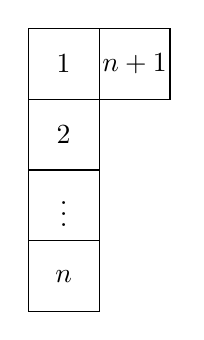
\begin{tikzpicture}[scale=0.9,baseline=-54pt]
	\hobox{0}{0}{1}
	\hobox{1}{0}{n+1}
	\hobox{0}{1}{2}
	\hobox{0}{2}{\vdots}
	\hobox{0}{3}{n}
	\end{tikzpicture}}.$$
By \cite[Thm. 5]{Bchen}, every element in this right cell $w_0\mathcal{C}_1$ is smooth. Thus from Proposition \ref{smoothequal} and Lemma \ref{constant} we have $V(L_w)=\mathcal{V}(w)=\mathcal{V}(w_0s_1)$ for any $w\in w_0\mathcal{C}_1$.

{\bf Case 2.} Similarly by \cite[Thm. 5]{Bchen}, every element $w$ in the right cell $w_0\mathcal{C}_{n}$ is smooth since $$P(w)=\small{
	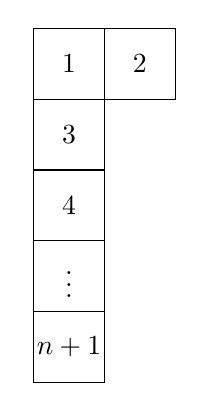
\begin{tikzpicture}[scale=0.9,baseline=-54pt]
	\hobox{0}{0}{1}
	\hobox{1}{0}{2}
	\hobox{0}{1}{3}
	\hobox{0}{2}{4}
	\hobox{0}{3}{\vdots}
        \hobox{0}{4}{n+1}
	\end{tikzpicture}}.$$
   Thus we have $V(L_w)=\mathcal{V}(w_0s_{n})$ for any $w\in w_0\mathcal{C}_{n}$.

{\bf Case 3.} For any  $1<i<n$ and $w\in w_0\mathcal{C}_{i}$, we have $$P(w)=P(w_0s_is_{i+1}\cdots s_{n})=\tiny{
	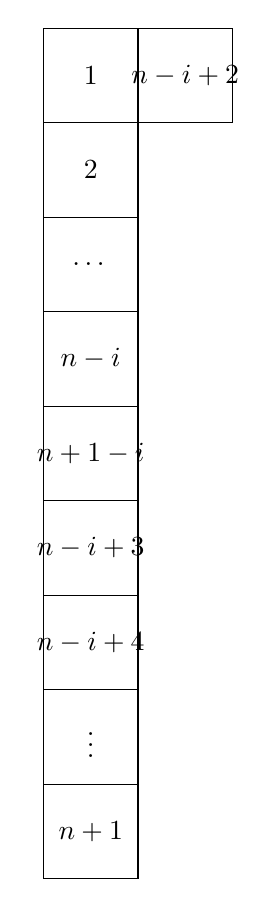
\begin{tikzpicture}[scale=1.2,baseline=-165pt]
	\hobox{0}{0}{1}
	\hobox{1}{0}{n-i+2}
	\hobox{0}{1}{2}
	\hobox{0}{2}{\dots}
	\hobox{0}{3}{n-i}
        \hobox{0}{4}{n+1-i}
        \hobox{0}{5}{n-i+3}
        \hobox{0}{6}{n-i+4}
        \hobox{0}{7}{\vdots}
        \hobox{0}{8}{n+1}
	\end{tikzpicture}}.$$
Note that \begin{align*}
    w_0s_is_{i+1}\cdots s_{k}=(&n+1,n,n-1,\cdots,n-i+3,n-i+1,n-i,\cdots,\\
&n-k+1, n-i+2,n-k,n-k-1,\cdots,2,1),
\end{align*} which has the  pattern $4231$ for $i\leq k\leq n-1$.



Note that \begin{align*}
    w_0s_is_{i-1}\cdots s_{k}=(&n+1,n,n-1,\cdots,n-k+3,n-i+1,n-k+2,\\
&n-k+1,\cdots,n-i+2,n-i,n-i-1,\cdots,2,1),
\end{align*} which has the  pattern $4231$ for $2\leq k\leq i$.

Also we have \begin{align*}
    w_0s_is_{i-1}\cdots s_{1}=(&n-i+1,n+1,n,n-1,\cdots,n-i+2,n-i,\\
    &n-i-1,\cdots,2,1),
\end{align*} which avoids the two patterns $4231$ and $3412$. Thus by Proposition \ref{3412}, the Schubert variety $X(w_0s_is_{i-1}\cdots s_{1})$ is smooth.


And $$w_0s_is_{i+1}\cdots s_{n}=(n+1,n,\cdots,n-i+3,n-i+1,n-i,\cdots,2,1,n-i+2),$$ which avoids the two patterns $4231$ and $3412$. Thus by Proposition \ref{3412}, the Schubert variety $X(w_0s_is_{i+1}\cdots s_{n})$ is smooth. 






Therefore, from  Lemma \ref{constant} we have $$V(L_w)=V(L_{w_0s_is_{i+1}\cdots s_{n}})=\mathcal{V}(w_0s_is_{i+1}\cdots s_{n})$$ for any $w\in w_0\mathcal{C}_{i}$.

For a right cell $\mathcal{R}$, we use $S(\mathcal{R})$ to denote the smooth elements contained in $\mathcal{R}$.
\begin{cor}
For type $A_{n}$,     we have $S(w_0\mathcal{C}_{1})=w_0\mathcal{C}_{1}$ and $S(w_0\mathcal{C}_{n})=w_0\mathcal{C}_{n}$.  When $2\leq i\leq n-1$, we have $$S(w_0\mathcal{C}_{i})=\{w_0s_is_{i-1}\cdots s_{1},w_0s_is_{i+1}\cdots s_{n}\}.$$
\end{cor}

\begin{cor}
   For type $A_{n}$ and $w\in w_0\mathcal{C}$, the associated variety of $L_w$ will be irreducible. We have $V(L_w)=\mathcal{V}(w_0s_is_{i+1}\cdots s_{n})=\mathcal{V}(w_0s_is_{i-1}\cdots s_{1})$ if  $w\in w_0\mathcal{C}_{i}$.
\end{cor}

From Proposition \ref{geometriccell}, for type $A_n$, we have $V(L_w)=\mathcal{V}(w_0s_i)=\mathcal{V}(w_{\rm max})$ if $w\in w_0\mathcal{C}_i$.





\section{The case of $C_n$ and $B_n$}\label{typebc}

In this section, we give the proof of our Theorem \ref{smcell} and Theorem \ref{AV-min} for types $B$ and $C$.


First we consider the case of type $C_n$.

\subsection{The case of $C_n$}We split the proof into several cases.

{\bf Case 1.} From Table \ref{Elements-in-cell} and Lemma \ref{long}, we have 
\begin{align*}
    w_0\mathcal{C}_1=\{&(-1,-2,\cdots,2-n,-n,1-n),\\
    &(-1,-2,\cdots,3-n,-n,2-n,1-n),\\
	&\vdots\\
    &(-n,-1,-2,\cdots,1-n),\\
	&(n,-1,-2,\cdots,1-n),\\
	&(-1,n,-2,\cdots,1-n),\\
	&\vdots\\
	&(-1,-2,\cdots,1-n,n)\}.
\end{align*}

% Thus for any $w\in w_0\mathcal{C}_1$, we have

% $$
% P(w)=
% 	\begin{tikzpicture}[scale=0.8,baseline=-125pt]
% 	\vdom{0}{1}{1}
% 	\vdom{0}{3}{2}
% 	\vdom{0}{5}{\cdots}
% 	\vdom{0}{7}{n-1}
% 	\vdom{1}{1}{n}	
% 	\end{tikzpicture}.
% $$

Next we prove that every element in this KL right cell $w_0\mathcal{C}_1$ is smooth. We use $[n, m]$ to denote the set $\{n, n + 1, ..., m\}$ for $n < m$. We use
“$k$” to denote the $k$-th largest element in a pattern and “$\bar{k}$” the opposite number of this element.

For $w_0\mathcal{C}_1$, we have 
\begin{align*}
    w_0s_1s_2\cdots s_k=(&-1,-2,\cdots,-n+k+1,-n,-n+k,\\&-n+k-1,\cdots,1-n)\text{~for~} 1\leq k\leq n-1
\end{align*}
 and 
 \begin{align*}
     w_0s_1s_2\cdots s_ns_{n-1}\cdots s_{n-j+1}=(&-1,-2,\cdots,1-j,n,-j,\\&-j-1,\cdots,1-n)\text{~for~}1\leq j\leq n.
 \end{align*}
 
 For the permutation $(-1,-2,\cdots,-n+k+1,-n,-n+k,-n+k-1,\cdots,1-n)$, we assert that the patterns $\bar{2}\bar{1}\bar{3}$, $\bar{3}\bar{2}\bar{1}$ and $\bar{3}\bar{4}\bar{1}\bar{2}$ can not appear. Note that the subsequence $(-1,-2,\cdots,-n+k+1,-n+k,-n+k-1,\cdots,1-n)$ is decreasing, then the pattern $\bar{2}\bar{1}\bar{3}$ and $\bar{3}\bar{2}\bar{1}$ can not appear. For the pattern $\bar{3}\bar{4}\bar{1}\bar{2}$, the element “$\bar{3}$” 
must be chosen from $[-n,-1]$ (since “$\bar{1}$” and “$\bar{2}$” are fixed at $[1-n,k-n]$). The relative order of “$\bar{3}$” and “$\bar{1}$” makes the pattern $\bar{3}\bar{4}\bar{1}\bar{2}$  impossible. 

For the permutation $(-1,-2,\cdots,1-j,n,-j,-j-1,\cdots,1-n)$, the discussion is similar and next we assert that the patterns $\bar{1}2\bar{3}$, $\bar{2}1\bar{3}$, $2\bar{1}\bar{3}$, $2\bar{3}\bar{1}$, $\bar{3}\bar{2}1$, $\bar{3}2\bar{1}$, $3\bar{2}\bar{1}$, $1\bar{2}$ can not appear. Note that the positive part of these eight patterns is fixed by $n$ and  the subsequence $(-1,-2,\cdots,1-j,-j,-j-1,\cdots,1-n)$ is decreasing, then the patterns $2\bar{3}\bar{1}$, $\bar{3}\bar{2}1$, $\bar{3}2\bar{1}$, $3\bar{2}\bar{1}$ can not appear. The remaining four patterns $\bar{1}2\bar{3}$, $\bar{2}1\bar{3}$, $2\bar{1}\bar{3}$ and $1\bar{2}$ can not appear since “1” is fixed by $n$, but there is no element larger than $n$ in this permutation. 

Therefore by Theorem \ref{pattern-avoid},  the Schubert variety $X(w)$  is smooth for each $w\in w_0\mathcal{C}_1$.

{\bf Case 2.} Similarly in the KL right cell $w_0\mathcal{C}_n$, we have 
$$w_0s_ns_{n-1}\cdots s_1=(-2,\cdots,-n,1),$$
which avoids the  $11$ patterns listed in Theorem \ref{pattern-avoid}, thus the Schubert variety $X(w_0s_ns_{n-1}\cdots s_1)$ is smooth. 


Also, we have
$$
w_0s_ns_{n-1}\cdots s_k=(-2,\cdots,-(n-k+1),1,-(n-k+2),\cdots,-n),
$$
which has the pattern $1\bar{2}$ for $1\leq k\leq n-1$ and so does $ w_0s_ns_{n-1}s_n=(2,1,-3,-4,\cdots,-n)$.

{\bf Case 3.} For any $1<i<n$ and $w\in w_0\mathcal{C}_i$, we have the following.
\begin{enumerate}
    \item  For $w=w_0s_is_{i-1}\cdots s_{i-k+1}$,
    \begin{enumerate}
        \item When $1\leq k\leq i-1$, we have
\begin{align*}
&w_0s_is_{i-1}\cdots s_{i-k+1}\\
=&(-1,-2,\cdots,-(n-i-1),-(n-i+1),\cdots,\\&-(n-i+k),-(n-i),-(n-i+k+1),\cdots,-n),
\end{align*}
which has the pattern $\bar{2}\bar{1}\bar{3}$.

\item  When $k=i$, we have
\begin{align*}
&w_0s_is_{i-1}\cdots s_{1}\\
=&(-1,-2,\cdots,-(n-i-1),-(n-i+1),\cdots,-n,-(n-i)),
\end{align*}
which avoids the $11$ patterns listed in Theorem \ref{pattern-avoid}. Thus the Schubert variety $X(w_0s_is_{i-1}\cdots s_1)$ is smooth.
    \end{enumerate}
    

\item  For $w=w_0s_is_{i+1}\cdots s_k$ with $i\leq k\leq n-1$, we have
\begin{align*}
&w_0s_is_{i+1}\cdots s_k\\
=&(-1,-2,\cdots,-(n-k-1),-(n-i+1),-(n-k),\\
&-(n-k+1),\cdots,-(n-i),-(n-i+2),\cdots,-n),
\end{align*}
which has the pattern $\bar{2}\bar{1}\bar{3}$.

\item For $w=w_0s_is_{i+1}\cdots s_ns_{n-1}\cdots s_{n-k+1}$,
\begin{enumerate}
    \item When $1\leq k\leq n-1$, we have
\begin{align*}
&w_0s_is_{i+1}\cdots s_ns_{n-1}\cdots s_{n-k+1}\\
=&(-1,-2,\cdots,-(k-1),n-i+1,-k,\\
&-(k+1),\cdots,-(n-i),-(n-i+2),\cdots,-n),
\end{align*}
which has the pattern $1\bar{2}$.

\item When $k=n$,  we have
\begin{align*}
&w_0s_is_{i+1}\cdots s_ns_{n-1}\cdots s_{1}\\
=&(-1,-2,\cdots,-(n-i),-(n-i+2),\cdots,-n,n-i+1),
\end{align*}
which avoids the $11$ patterns listed in Theorem \ref{pattern-avoid}. Thus the Schubert variety $X(w_0s_is_{i+1}\cdots s_ns_{n-1}\cdots s_{1})$ is smooth.
    
\end{enumerate}


\end{enumerate}




% \begin{align*}
% w_0s_is_{i-1}\cdots s_{i-k+1}=(&-1,-2,\cdots,-(n-i-1),-(n-i+1),\cdots,-(n-i+k),\\&-(n-i),-(n-i+k+1),\cdots,-n),
% \end{align*}
% which has the pattern $\bar{2}\bar{1}\bar{3}$ for $1\leq k\leq i-1$. When $k=i$ we have
% \begin{align*}
% w_0s_is_{i-1}\cdots s_{1}=(&-1,-2,\cdots,-(n-i-1),-(n-i+1),\cdots,-n,-(n-i)),
% \end{align*}
% which avoids 11 patterns listed in Theorem \ref{pattern-avoid} for $1<i<n$. Thus the Schubert variety $X(w_0s_is_{i-1}\cdots s_1)$ is smooth.

% Note that
% \begin{align*}
% w_0s_is_{i+1}\cdots s_k=(&-1,-2,\cdots,-(n-k-1),-(n-i+1),-(n-k),\\&-(n-k+1),\cdots,-(n-i),-(n-i+2),\cdots,-n),
% \end{align*}
% which has the pattern $\bar{2}\bar{1}\bar{3}$ for $i\leq k\leq n-1$.

% Also we have
% \begin{align*}
% w_0s_is_{i+1}\cdots s_ns_{n-1}\cdots s_{n-k+1}=(&-1,-2,\cdots,-(k-1),n-i+1,-k,\\&-(k+1),\cdots,-(n-i),-(n-i+2),\cdots,-n),
% \end{align*}
% which has the pattern $1\bar{2}$ for $1\leq k\leq n-1$.

% Note that
% \begin{align*}
% w_0s_is_{i+1}\cdots s_ns_{n-1}\cdots s_{1}=(-1,-2,\cdots,-(n-i),-(n-i+2),\cdots,-n,n-i+1),
% \end{align*}
% which avoids 11 patterns listed in Theorem \ref{pattern-avoid}. Thus the Schubert variety $X(w_0s_is_{i+1}\cdots s_ns_{n-1}\cdots s_{1})$ is smooth.

\begin{cor}
    For type $C_n$, we have $S(w_0\mathcal{C}_1)=w_0\mathcal{C}_1$ and  $S(w_0\mathcal{C}_n)=\{w_0s_ns_{n-1}\cdots s_1\}$.  When $1<i< n$, we have 
    $$S(w_0\mathcal{C}_i)=\{w_0s_is_{i-1}\cdots s_1, w_0s_is_{i+1}\cdots s_ns_{n-1}\cdots s_{1}\}.$$
\end{cor}

\begin{cor}
    When $W=W(C_n)$ and $w\in w_0\mathcal{C}$, the associated variety of $L_w$ will be irreducible. We have $V(L_w)=\mathcal{V}(w_0s_is_{i+1}\cdots s_ns_{n-1}\cdots s_{1})$ if $w\in w_0\mathcal{C}_i$.
\end{cor}

Note that $w_0s_is_{i+1}\cdots s_ns_{n-1}\cdots s_{1}$ is the minimal length element $w_{\rm min} $
 of the KL right cell $w_0\mathcal{C}_i$.
 
\subsection{The case of $B_n$}
Now we consider the case of type $B_n$. The result for type $B_n$ can be obtained by adapting the argument for type $C_n$, since they share the same Weyl group. From \cite[Thm. 4.2 and Thm. 6.1]{Bi-98} we divide the discussion into the following three cases:
\begin{enumerate}
    \item[(i)] If $X(w)$ is not smooth in type $C_n$ and $w$ contains one of the patterns listed in \cite[Thm. 4.2]{Bi-98}, then $X(w)$ is not smooth in type $B_n$;

    \item[(ii)] If $X(w)$ is not smooth in type $C_n$ and $w$ contains only the pattern $1\bar{2}$, then to determine whether $X(w)$ is smooth in type $B_n$, it suffices to check whether $w$ avoids the pattern $\bar{2}\bar{1}$;

    \item[(iii)] If $X(w)$ is smooth in type $C_n$, which means that $w$ avoids the patterns listed in \cite[Thm. 4.2 and Thm. 6.1]{Bi-98}, then it again suffices to check whether $w$ avoids the pattern $\bar{2}\bar{1}$.
\end{enumerate}
% In what follows, we only consider the cases (ii) and (iii).


% Recall that in the case of type $C_n$, there are three cases.    if $X(w)$ is smooth, or if it is non-smooth since $w$ only has the pattern $1\bar{2}$, then $w\in w_0\mathcal{C}_i$ avoids the patterns listed in \cite[(13.3.4)]{Bi-98}. To determine whether $X(w)$ is smooth in type $B_n$, it suffices to check whether $w$ avoids the pattern $\bar{2}\bar{1}$.

{\bf Case 1.} For the KL right cell $ w_0\mathcal{C}_1$, we have $S( w_0\mathcal{C}_1)= w_0\mathcal{C}_1$ in the case of $C_n$, then we only need to check the pattern $\bar{2}\bar{1}$ in the case of type $B_n$.

For $w\in w_0\mathcal{C}_1$, we have 
\begin{align*}
    w_0s_1s_2\cdots s_k=(&-1,-2,\cdots,-n+k+1,-n,-n+k,\\&-n+k-1,\cdots,1-n)\text{~for~} 1\leq k\leq n-1
\end{align*}
 and 
 \begin{align*}
     w_0s_1s_2\cdots s_ns_{n-1}\cdots s_{n-j+1}=(&-1,-2,\cdots,1-j,n,-j,\\&-j-1,\cdots,1-n)\text{~for~}1\leq j\leq n.
 \end{align*}

For the permutation of $(-1,-2,\cdots,-n+k+1,-n,-n+k,-n+k-1,\cdots,1-n)$, it has the pattern $\bar{2}\bar{1}$ for $1\leq k \leq n-1$. For the permutation $(-1,-2,\cdots,1-j,n,-j,-j-1,\cdots,1-n)$, it avoids the pattern $\bar{2}\bar{1}$ for $1\leq j\leq n$ since the subsequence $(-1,-2,\cdots,1-j,-j,-j-1,\cdots,1-n)$ is decreasing, the relative order of “$\bar{2}$” and “$\bar{1}$” makes the pattern $\bar{2}\bar{1}$ impossible. 

{\bf Case 2.} Similarly for the KL right cell $w_0\mathcal{C}_n$, we have $S(w_0\mathcal{C}_n)=\{w_0s_ns_{n-1}\cdots s_1\}$ in the case of $C_n$. Note that 
$$w_0s_ns_{n-1}\cdots s_1=(-2,\cdots,-n,1),$$
which avoids the pattern $\bar{2}\bar{1}$, thus by Theorem \ref{pattern-avoid}  the Schubert variety $X(w_0s_ns_{n-1}\cdots s_1)$ is smooth.  \\
We also have
\begin{align*}
w_0s_ns_{n-1}\cdots s_k=(-2,\cdots,-(n-k+1),1,-(n-k+2),\cdots,-n),
\end{align*}
which has the pattern $\bar{2}1\bar{3}$ for $2\leq k\leq n-1$, and  
$$w_0s_ns_{n-1}s_n=(2,1,-3,-4,\cdots,-n)$$
has the pattern $1\bar{2}\bar{3}$.

{\bf Case 3.} For any $1<i<n$ and $w\in w_0\mathcal{C}_i$, we have the following.
\begin{enumerate}
    \item For $w=w_0s_is_{i-1}\cdots s_{i-k+1}$, when $1\leq k\leq i$ we have
\begin{align*}
&w_0s_is_{i-1}\cdots s_{i-k+1}\\
=&(-1,-2,\cdots,-(n-i-1),-(n-i+1),\cdots,-(n-i+k),\\
&-(n-i),-(n-i+k+1),\cdots,-n),
\end{align*}
which has the pattern $\bar{2}\bar{1}$.

\item For $w=w_0s_is_{i+1}\cdots s_k$, when $i\leq k\leq n-1$ we have
\begin{align*}
&w_0s_is_{i+1}\cdots s_k\\
=&(-1,-2,\cdots,-(n-k-1),-(n-i+1),-(n-k),\\&-(n-k+1),\cdots,-(n-i),-(n-i+2),\cdots,-n),
\end{align*}
which has the pattern $\bar{2}\bar{1}$.

\item For $w=w_0s_is_{i+1}\cdots s_ns_{n-1}\cdots s_{n-k+1}$,
\begin{enumerate}
    \item When $k=1$, we have
    \begin{align*}
w_0s_is_{i+1}\cdots s_n=(n-i+1,-1,-2,\cdots,-(n-i),-(n-i+2),\cdots,-n),
\end{align*}
which has the pattern  $2\bar{1}\bar{3}$.

\item When $2\leq k\leq n-1$, we have
\begin{align*}
&w_0s_is_{i+1}\cdots s_ns_{n-1}\cdots s_{n-k+1}\\
=&(-1,-2,\cdots,-(k-1),n-i+1,-k,\\&-(k+1),\cdots,-(n-i),-(n-i+2),\cdots,-n),
\end{align*}
which has the pattern $\bar{1}2\bar{3}$.

\item When $k=n$, we have
\begin{align*}
&w_0s_is_{i+1}\cdots s_ns_{n-1}\cdots s_1\\
=&(-1,-2,\cdots,-(n-i),-(n-i+2),\cdots,-n,n-i+1),
\end{align*}
which avoids the pattern $\bar{2}\bar{1}$, thus by Theorem \ref{pattern-avoid} the Schubert variety $X(w_0s_is_{i+1}\cdots s_ns_{n-1}\cdots s_{n-i+1})$ is smooth.
    
\end{enumerate}



    
\end{enumerate}



% \begin{align*}
% w_0s_is_{i-1}\cdots s_{i-k+1}=(&-1,-2,\cdots,-(n-i-1),-(n-i+1),\cdots,-(n-i+k),\\&-(n-i),-(n-i+k+1),\cdots,-n),
% \end{align*}
% which has the pattern $\bar{2}\bar{1}$ for $1\leq k\leq i$.

% Note that
% \begin{align*}
% w_0s_is_{i+1}\cdots s_k=(&-1,-2,\cdots,-(n-k-1),-(n-i+1),-(n-k),\\&-(n-k+1),\cdots,-(n-i),-(n-i+2),\cdots,-n),
% \end{align*}
% which has the pattern $\bar{2}\bar{1}$ for $i\leq k\leq n-1$.

% Also we have
% \begin{align*}
% w_0s_is_{i+1}\cdots s_ns_{n-1}\cdots s_{n-k+1}=(&-1,-2,\cdots,-(k-1),n-i+1,-k,\\&-(k+1),\cdots,-(n-i),-(n-i+2),\cdots,-n),
% \end{align*}
% which has the pattern $\bar{1}2\bar{3}$ for $2\leq k\leq n-1$ and the pattern $2\bar{1}\bar{3}$ for $k=1$.

% Note that
% \begin{align*}
% w_0s_is_{i+1}\cdots s_ns_{n-1}\cdots s_1=(-1,-2,\cdots,-(n-i),-(n-i+2),\cdots,-n,n-i+1),
% \end{align*}
% which avoids the pattern $\bar{2}\bar{1}$, thus by Theorem \ref{pattern-avoid} the Schubert variety $X(w_0s_ns_{n-1}\cdots s_{n-i+1})$ is smooth.

\begin{cor}
    For type $B_n$, we have $$S(w_0\mathcal{C}_1)=\{w_0s_1\cdots s_ns_{n-1}\cdots s_{n-j+1}\mid 1\leq j\leq n\}$$ and  $$S(w_0\mathcal{C}_n)=\{w_0s_ns_{n-1}\cdots s_1\}.$$   When $1<i< n$, we have 
    $$S(w_0\mathcal{C}_i)=\{w_0s_is_{i+1}\cdots s_ns_{n-1}\cdots s_1\}.$$
\end{cor}

\begin{cor}
    When $W=W(B_n)$ and $w\in w_0\mathcal{C}$, the associated variety of $L_w$ will be irreducible. We have 
$V(L_w)=\mathcal{V}(w_0s_is_{i+1}\cdots s_ns_{n-1}\cdots s_1)$ if $w\in w_0\mathcal{C}_i$.
\end{cor}

Note that $w_0s_is_{i+1}\cdots s_ns_{n-1}\cdots s_{1}$ is the minimal length element $w_{\rm min} $
 of the KL right cell $w_0\mathcal{C}_i$.



\section{The case of $D_n$}\label{typed}

In this section, we give the proof of our Theorem \ref{smcell} and Theorem \ref{AV-min} for type $D$.

Before proving our results, we have the following special case.
\begin{prop}\label{non-smooth}
    For type $D_n$ $(n\geq 4)$, all elements of the following KL right cells are non-smooth: $\{w_0\mathcal{C}_i\mid 2\leq i \leq n-2\}$.
\end{prop}
\begin{proof}
{\bf Case 1.} Suppose that $n$ is even.

    Note that 
    \begin{align*}
        &w_0s_is_{i-1}\cdots s_k\\
        =&(-1,\cdots,-(n-i-1),-(n-i+1),\cdots,-(n-i+k+1),\\&-(n-i),-(n-i+k+2),\cdots,-n),
    \end{align*}
which has the pattern $\bar{1}\bar{3}\bar{2}$ for $1\leq k\leq i-1$.

For the permutation 
\begin{align*}
    &w_0s_is_{i+1}\cdots s_{n-2}s_n\\=&(n-i+1,1,-2,\cdots,-(n-i-1),-(n-i),\\&-(n-i+2),\cdots,-n),
\end{align*}
which has the pattern $31\bar{2}\bar{4}$.

 Note that 
    \begin{align*}
        &w_0s_is_{i+1}\cdots s_{i+(k-1)}\\
        =&(-1,\cdots,-(n-i-k),-(n-i+1),-(n-i-k+1),\\&-(n-i-k+2),\cdots,-(n-i),-(n-i+2),\cdots,-n),
    \end{align*}
which has the pattern $\bar{1}\bar{3}\bar{2}$ for $2\leq k\leq n-i$ and the pattern $\bar{2}\bar{1}\bar{3}$ for $k=1$.

{\bf Case 2.} Suppose that $n$ is odd.

  Note that 
    \begin{align*}
        &w_0s_is_{i-1}\cdots s_k\\
        =&(1,\cdots,-(n-i-1),-(n-i+1),\cdots,-(n-i+k+1),\\&-(n-i),-(n-i+k+2),\cdots,-n),
    \end{align*}
which has the pattern $1\bar{3}\bar{2}$ for $1\leq k\leq i-1$.   

For the permutation 
\begin{align*}
    w_0s_is_{i+1}\cdots s_{n-2}s_n=(&-(n-i+1),1,-2,\cdots,-(n-i-1),-(n-i),\\&-(n-i+2),\cdots,-n),
\end{align*}
 which has the pattern $\bar{2}\bar{1}\bar{3}$.

 Note that 
    \begin{align*}
        &w_0s_is_{i+1}\cdots s_{i+(k-1)}\\
        =&(1,\cdots,-(n-i-k),-(n-i+1),-(n-i-k+1),\\&-(n-i-k+2),\cdots,-(n-i),-(n-i+2),\cdots,-n),
    \end{align*}
which has the pattern $1\bar{3}\bar{2}$ for $2\leq k\leq n-i$ and the pattern $3\bar{1}\bar{2}\bar{4}$ for $k=1$.

\end{proof}


For the remaining cases, we split the discussion into two subcases based on the parity of \(n\).
\subsection{Proof for even $n$}

{\bf Case 1.} From Table \ref{Elements-in-cell} and Lemma \ref{long}, we have 
\begin{align*}
    w_0\mathcal{C}_1=\{&(-1,-2,\cdots,2-n,-n,1-n),\\
	&\vdots\\
    &(-n,-1,-2,\cdots,1-n),\\
	&(n,1,-2,\cdots,1-n)\}.
\end{align*}

For the first $n-2$ permutations, they have the pattern $\bar{1}\bar{3}\bar{2}$. Next we prove that the last two permutations avoid the  $11$ patterns listed in Theorem \ref{pattern-avoid}.

For the permutation $(-n,-1,-2,\cdots,1-n)$, we only need to check the patterns $\bar{3}\bar{4}\bar{1}\bar{2}$, $\bar{1}\bar{3}\bar{2}$, $\bar{2}\bar{1}\bar{3}$ and $\bar{3}\bar{2}\bar{1}$. For the pattern $\bar{3}\bar{4}\bar{1}\bar{2}$, the element “$\bar{1}$” and “$\bar{2}$”  
must be chosen from $[1-n,-1]$. The relative order of “$\bar{3}$” and “$\bar{4}$” makes the pattern $\bar{3}\bar{4}\bar{1}\bar{2}$  impossible. For the pattern $\bar{1}\bar{3}\bar{2}$, the element “$\bar{1}$” and “$\bar{3}$”  
must be chosen from $[-n,-1]$, but there is no larger element “$\bar{2}$” such that “$\bar{2}$” is on the right side of  “$\bar{3}$”, thus the relative order of “$\bar{2}$” and “$\bar{3}$” makes the pattern $\bar{1}\bar{3}\bar{2}$ impossible. Similarly for the patterns $\bar{2}\bar{1}\bar{3}$ and $\bar{3}\bar{2}\bar{1}$, the relative order of “$\bar{2}$” and “$\bar{1}$" makes them impossible.

{\bf Case 2.} For $ w_0\mathcal{C}_{i}$ with $2\leq i\leq n-2$, we have given the result in Proposition \ref{non-smooth}.

{\bf Case 3.} For $ w_0\mathcal{C}_{n-1}$, we have
   $$ w_0s_{n-1}s_{n-2}s_n=(3,2,-1,-4,\cdots,-n),$$
which has the pattern $21\bar{3}\bar{4}$.

Also we have $$w_0s_{n-1}s_{n-2}\cdots s_k=(-2,\cdots,-k,-1,-k-1,\cdots,-n),$$
which has the pattern $\bar{2}\bar{1}\bar{3}$ for $2\leq k\leq n-1$. Note that $$w_0s_{n-1}s_{n-2}\cdots s_1=(-2,\cdots,-n,-1),$$ which avoids the $11$ patterns listed in Theorem \ref{pattern-avoid}, thus the Schubert variety $X(w_0s_{n-1}s_{n-2}\cdots s_1)$ is smooth.

{\bf Case 4.} For $w_0\mathcal{C}_{n}$, we have
   $$ w_0s_ns_{n-2}s_{n-1}=(-3,2,1,-4,\cdots,-n),$$
which has the pattern $21\bar{3}\bar{4}$.

Also we have $$w_0s_{n}s_{n-2}\cdots s_k=(2,-3,\cdots,-k,1,-k-1,\cdots,-n),$$
which has the pattern $2\bar{3}1\bar{4}$ for $3\leq k\leq n-1$ and $21\bar{3}\bar{4}$ for $k=2$. Note that $$w_0s_{n}s_{n-2}\cdots s_1=(2,-3,\cdots,-n,1),$$ which avoids the $11$ patterns listed in Theorem \ref{pattern-avoid}, thus the Schubert variety $X(w_0s_{n}s_{n-2}\cdots s_1)$ is smooth.

\subsection{Proof for odd $n$}

{\bf Case 1.} From Table \ref{Elements-in-cell} and Lemma \ref{long}, we have 
\begin{align*}
    w_0\mathcal{C}_1=\{&(1,-2,\cdots,2-n,-n,1-n),\\
	&\vdots\\
    &(n,-1,-2,\cdots,1-n),\\
	&(-n,1,-2,\cdots,1-n)\}.
\end{align*}

For the first $n-2$ permutations, they contain the pattern $1\bar{3}\bar{2}$, and the last two permutations avoid the $10$ patterns listed in Theorem \ref{pattern-avoid}. The argument is similar to the case where $n$ is even, so we omit the details here.

{\bf Case 2.} For $ w_0\mathcal{C}_{i}$ with $2\leq i\leq n-2$, we have given the result in
Proposition \ref{non-smooth}.

{\bf Case 3.} For $ w_0\mathcal{C}_{n-1}$, we have
   $$ w_0s_{n-1}s_{n-2}s_n=(-3,2,-1,-4,\cdots,-n),$$
which has the pattern $\bar{2}\bar{1}\bar{3}$.

Also we have $$w_0s_{n-1}s_{n-2}\cdots s_k=(2,-3,\cdots,-k,-1,-k-1,\cdots,-n),$$
which has the pattern $\bar{2}\bar{1}\bar{3}$ for $2\leq k\leq n-1$. When $k=1$ we have $$w_0s_{n-1}s_{n-2}\cdots s_1=(2,-3,\cdots,-n,-1),$$ which avoids the $10$ patterns listed in Theorem \ref{pattern-avoid}, thus the Schubert variety $X(w_0s_{n-1}s_{n-2}\cdots s_1)$ is smooth.

{\bf Case 4.} For $ w_0\mathcal{C}_{n}$, we have
   $$ w_0s_ns_{n-2}s_{n-1}=(3,2,1,-4,\cdots,-n),$$
which has the pattern $21\bar{3}\bar{4}$.

Also we have $$w_0s_{n}s_{n-2}\cdots s_k=(-2,-3,\cdots,-k,1,-k-1,\cdots,-n),$$
which has the pattern $\bar{2}\bar{3}1\bar{4}$ for $3\leq k\leq n-1$ and $\bar{2}1\bar{3}\bar{4}$ for $k=2$. When $k=1$ we have $$w_0s_{n}s_{n-2}\cdots s_1=(-2,-3,\cdots,-n,1),$$ which avoids the $10$ patterns listed in Theorem \ref{pattern-avoid}, thus the Schubert variety $X(w_0s_{n}s_{n-2}\cdots s_1)$ is smooth.
\begin{Rem}
   In types $D_3$ and $D_4$, in addition to the aforementioned smooth elements, there are additional smooth ones in $w_0\mathcal{C}_{n-1}$ and $w_0\mathcal{C}_{n}$:
    \smallskip
\begin{center}
\begin{tabular}{c|c|c}
\hline
 Lie type  &  $w_0\mathcal{C}_{n-1}$ &  $w_0\mathcal{C}_{n}$ \\
%\hline
\hline
\mystrut
$D_3$  & $w_0s_{2}s_{1}s_3$, $w_0s_{2}$ & $w_0s_{3}s_{1}s_2$, $w_0s_{3}$ \\[.05in]
\hline
\mystrut
$D_4$ & $w_0s_{3}s_{2}s_4$ & $w_0s_4s_2s_3$
   \\[.05in]
\hline


\end{tabular}
\end{center}
\medskip
\end{Rem}

\begin{cor}\label{smooth}
    % For type $D_n$, we have $$S(w_0\mathcal{C}_1)=\{w_0s_1\cdots s_{n-2}s_{n-1}, w_0s_1\cdots s_{n-2}s_{n}\}$$ if $n\geq 2$. When $n\geq 5$, we have $S(w_0\mathcal{C}_{n-1})=\{w_0s_{n-1}s_{n-2}\cdots s_1\}$, and $S(w_0\mathcal{C}_n)=\{w_0s_{n}s_{n-2}\cdots s_1\}$.
    For type $D_n$ ($n\geq 4$), we have  
$$S(w_0\mathcal{C}_1)=\{w_0s_1\cdots s_{n-2}s_{n-1},\; w_0s_1\cdots s_{n-2}s_{n}\}.$$  
Moreover, for $n\geq 5$, we have $$S(w_0\mathcal{C}_{n-1})=\{w_0s_{n-1}s_{n-2}\cdots s_1\}$$ and $$S(w_0\mathcal{C}_n)=\{w_0s_{n}s_{n-2}\cdots s_1\}.$$
\end{cor}

\begin{prop}
    When $W=W(D_n)$ with $n\geq 5$ and $w\in w_0\mathcal{C}_i$ for $1\leq i\leq n$, we have 
    \[{
V(L_w)=
\begin{cases}
\mathcal V(s_1w_0)=\mathcal V(w_0s_1)=\mathcal V(w_0s_1\cdots s_{n-2}s_{n-1}) & \text{if~}i=1;\\
\mathcal V(s_iw_0)=\mathcal V(w_0s_i)=\mathcal V(w_0s_is_{i+1}\cdots s_{n-1})  & \text{if~} 2\leq i\leq n-2\\
&\text{~and~}n-i\geq i;\\
\mathcal V(s_iw_0)=\mathcal V(w_0s_i)=\mathcal V(w_0s_is_{i-1}\cdots s_{1})  & \text{if~} 2\leq i\leq n-2\\
&\text{~and~}n-i< i;\\
\mathcal V(w_0s_{n-1})= \mathcal V(w_0s_{n-1}s_{n-2}\cdots s_1)& \text{if~}i=n-1;\\
\mathcal V(w_0s_{n})=\mathcal V(w_0s_{n}s_{n-2}\cdots s_1) & \text{if~}i=n.
\end{cases}}
\]
% \begin{align*}
% &V(L_w)=\\
% &\begin{cases}
% \begin{aligned}
% \mathcal V(s_1w_0) &= \mathcal V(w_0s_1) \\
% &= \mathcal V(w_0s_1\cdots s_{n-2}s_{n-1})
% \end{aligned} & \text{if } i=1;\\[4pt]
% \begin{aligned}
% \mathcal V(s_iw_0) &= \mathcal V(w_0s_i) \\
% &= \mathcal V(w_0s_is_{i+1}\cdots s_{n-1})
% \end{aligned} & \text{if } 2\leq i\leq n-2 \text{ and } n-i\geq i;\\[4pt]
% \begin{aligned}
% \mathcal V(s_iw_0) &= \mathcal V(w_0s_i) \\
% &= \mathcal V(w_0s_is_{i-1}\cdots s_{1})
% \end{aligned} & \text{if } 2\leq i\leq n-2 \text{ and } n-i< i;\\[4pt]
% \begin{aligned}
% \mathcal V(w_0s_{n-1}) &= \mathcal V(w_0s_{n-1}s_{n-2}\cdots s_1)
% \end{aligned} & \text{if } i=n-1;\\[4pt]
% \begin{aligned}
% \mathcal V(w_0s_{n}) &= \mathcal V(w_0s_{n}s_{n-2}\cdots s_1)
% \end{aligned} & \text{if } i=n.
% \end{cases}
% \end{align*}


\end{prop}
\begin{proof}
  Suppose $w\in w_0\mathcal{C}_i$. If the right cell $w_0\mathcal{C}_i$ contains some smooth element $w_0x$, we will have $V(L_w)=V(L_{w_0x})=\mathcal{V}(w_0x)$ for any $w\in w_0\mathcal{C}_i$ by Lemma \ref{constant} and Proposition \ref{smoothequal}. Thus 
$V(L_{w})$ can be characterized by Corollary \ref{smooth} for $i=1, n-1$ and $n$.

 


From \cite[\S 2.3 and Exer. 4.10]{BB05}, we have $$w_0s_i=\begin{cases}
s_iw_0 &  \text{~if~} 1\leq i\leq n-2;\\
s_{n-1}w_0  &  \text{~if~$n$~is~even, and~} i=n-1;\\
s_{n}w_0  &  \text{~if~$n$~is~odd, and~} i=n-1;\\
s_{n}w_0  &  \text{~if~$n$~is~even, and~} i=n;\\
s_{n-1}w_0  &  \text{~if~$n$~is~odd, and~} i=n.
\end{cases}$$

 When $i=1$, similarly we also have $V(L_w)=\mathcal V(s_1w_0)=\mathcal V(w_0s_1)$.

 But when $i=n-1$, from Lemma \ref{minimal-integralequal} we have 
 $V(L_w)=\mathcal V(s_{n-1}w_0)=\mathcal V(w_0s_{n-1})$ when $n$ is even and $V(L_w)=\mathcal V(s_{n}w_0)=\mathcal V(w_0s_{n-1})$ when $n$ is odd. When $i=n$, the result is similar.

 Next, we consider the case where there is no smooth element in $w_0\mathcal{C}_i$ for $2\leq i\leq n-2$. 
 
 When $w \in w_0\mathcal{C}_i$ with $2\leq i\leq n-2$, Lemma \ref{constant} implies $V(L_w) = V(L_{w_i})$, where  $w_i=w_0s_is_{i+1}\cdots s_{n-1}$ if $n-i\geq i$ and $w_i=w_0s_is_{i-1}\cdots s_{1}$ if $n-i\leq i$.
 \begin{enumerate}
     \item When $n$ is even  and $n-i\geq i$, we have $w_0(\alpha_i)=-\alpha_i$. In this case $w_i=w_0s_is_{i+1}\cdots s_{n-1}$ is the minimal length element in the right cell $w_0\mathcal{C}_i$. From Lemma \ref{gamma-w} we have $V(L_{w_i})=\bigcup\limits_{y\in \Gamma(w_i)}\mathcal{V}(y)$ for some subset $\Gamma(w_i)\subset W$.  Also  for any $y\in \Gamma(w_i)$, we have  
     \begin{equation}\label{orbital-element}
    y\leq w_i \text{~and~} y\in w_0\mathcal{C}.
     \end{equation}
There are $i$ elements which may satisfy the condition (\ref{orbital-element}): $$w_i,w_{i-1},\cdots, w_1,$$ where $w_t=w_0s_ts_{t+1}\cdots s_{n-1}\in w_0\mathcal{C}_t$ for $1\leq t\leq i$. We claim that 
     \begin{align}\label{Gamma-set}
         \Gamma(w_t)=w_t.
     \end{align}
We prove the claim (\ref{Gamma-set}) by induction on $t$. If $t=1$, $w_1$ is minimal length element in two-sided cell $w_0\mathcal{C}$, then $ \Gamma(w_1)=w_1$ by Lemma \ref{min-length-w}. If $t=2$, there are only two elements which may satisfy the condition (\ref{orbital-element}): $w_2$ and $w_1$. Denote ${\rm J}_l=\Pi\setminus {\alpha_l}$. First we have $-w_0s_2\rho=-w_0(\rho-\alpha_2)=\rho-\alpha_2$, which is $\Phi_{{\rm J}_{2}}^+$-dominant. Then from Proposition \ref{Same}, $V(L_{w_2})=V(L_{w_0s_2})\subset \fru_{\operatorname{J}_2}$ since $w_0s_2\in w_0\mathcal{C}_2$. If $w_1\in\Gamma(w_2)$, we will have $V(L_{w_1})=\mathcal{V}(w_1)\subset V(L_{w_2})\subset \fru_{\operatorname{J}_2}$. Then from Proposition \ref{Same}, $-w_0s_1\rho=\rho-\alpha_1$ will be  $\Phi_{{\rm J}_2}^+$-dominant, which is a contradiction since $(\rho-\alpha_1,\alpha^{\vee}_1)=-1$. Thus $\Gamma(w_2)=w_2$. Now assume that for $t\leq i-1$, we always have $\Gamma(w_{t})=w_{t}$. When $t=i$, $-w_0s_i\rho=-w_0(\rho-\alpha_i)=\rho-\alpha_{i}$ is $\Phi_{{\rm J}_{i}}^+$-dominant. Then $V(L_{w_i})=V(L_{w_0s_i})\subset \fru_{\operatorname{J}_i}$ since $w_0s_i\in w_0\mathcal{C}_i$. If $w_k=s_ks_{k+1}\cdots s_{n-1}\in\Gamma(w_i)$ for some $1\leq k<i$, we will have $V(L_{w_k})=\mathcal{V}(w_k)\subset V(L_{w_i})\subset\fru_{\operatorname{J}_i}$. Then from Proposition \ref{Same}, $-w_0s_k\rho=\rho-\alpha_k$ will be  $\Phi_{{\rm J}_i}^+$-dominant, which is a contradiction since $(\rho-\alpha_k,\alpha^{\vee}_k)=-1$. Thus $w_k\notin \Gamma(w_i)$. So we must have $\Gamma(w_i)=w_i$.

\item When $n$ is even  and $n-i< i$, we have $w_0(\alpha_i)=-\alpha_i$. In this case $w_i=w_0s_is_{i-1}\cdots s_{1}$ is the minimal length element in the right cell $w_0\mathcal{C}_i$. There are $n-i$ elements which may satisfy the condition (\ref{orbital-element}): $w_i,w_{i+1},\cdots, w_n$, where $w_t=w_0s_ts_{t-1}\cdots s_1\in w_0\mathcal{C}_t$ for $i\leq t\leq n$. First we have $-w_0s_i\rho=-w_0(\rho-\alpha_i)=\rho-\alpha_{i}$, which is $\Phi_{{\rm J}_{i}}^+$-dominant. Then $V(L_{w_i})=V(L_{w_0s_i})\subset \fru_{\operatorname{J}_i}$ since $w_0s_i\in w_0\mathcal{C}_i$. Similarly we start the induction process from $t=n$ and assume that for $i-1\leq t\leq n$, we always have $\Gamma(w_{t})=w_{t}$. 
When $t=i$, $-w_0s_i\rho=-w_0(\rho-\alpha_i)=\rho-\alpha_{i}$ is $\Phi_{{\rm J}_{i}}^+$-dominant. Then $V(L_{w_i})=V(L_{w_0s_i})\subset \fru_{\operatorname{J}_i}$ since $w_0s_i\in w_0\mathcal{C}_i$. If $w_k=s_ks_{k-1}\cdots s_{1}\in\Gamma(w_i)$ for some $i-1\leq k\leq n$, we will have $V(L_{w_k})=\mathcal{V}(w_k)\subset V(L_{w_i})\subset\fru_{\operatorname{J}_i}$. Then from Proposition \ref{Same}, $-w_0s_k\rho=\rho-\alpha_k$ will be  $\Phi_{{\rm J}_i}^+$-dominant, which is a contradiction since $(\rho-\alpha_k,\alpha^{\vee}_k)=-1$. Thus $w_k\notin \Gamma(w_i)$. So we must have $\Gamma(w_i)=w_i$.




% If $w_l=w_0s_ls_{l-1}\cdots s_1\in\Gamma(w_i)$ for $i< l\leq n$, similarly we will have $\Gamma(w_l)=w_l$ if we prove by induction on $l$. Then $V(L_{w_l})=\mathcal{V}(w_l)\subset V(L_{w_i})\subset\fru_{\operatorname{J}_i}$. Then from Proposition \ref{Same}, $-w_0s_l\rho=\rho-\alpha_k$ will be  $\Phi_{{\rm J}_i}^+$-dominant, which is a contradiction since $(\rho-\alpha_l,\alpha^{\vee}_l)=-1$. Thus $w_l\notin \Gamma(w_i)$. So we must have $\Gamma(w_i)=w_i$.

\item When $n$ is odd, we will have 
\[
w_0(\alpha_i)=-\alpha_{k_i}=\begin{cases}
    -\alpha_i, & \text{~if~} 1\leq i\leq n-2,\\
    -\alpha_n,& \text{~if~} i=n-1,\\
    -\alpha_{n-1}, &\text{~if~} i=n.
\end{cases}
\]




In this case, the argument is similar to the case when $n$ is even, so we omit the details here. Then we obtain $\Gamma(w_i) = w_i$.

 \end{enumerate}
 
 On the other hand, it is easy to check that $(-w_0s_i\rho,\alpha_{k_i}^{\vee})=(\rho-\alpha_{k_i},\alpha_{k_i}^{\vee})=0$  and $(-w_0s_i\rho,\alpha_j^{\vee})>0$ for all $j\neq k_i$, then by Lemma \ref{minimal-integralequal} we have $V(L_w)=V(L_{w_0s_i})=\mathcal V(s_{k_i}w_0)=\mathcal V(w_0s_i)$ for $w\in w_0\mathcal{C}_i$.



 
\end{proof}

Note that  the minimal length element 
 of the KL right cell $w_0\mathcal{C}_i$ is 
 $$w_{\rm min}=\begin{cases}
w_0s_1\cdots s_{n-2}s_{n-1} & \text{if~}i=1;\\
w_0s_is_{i+1}\cdots s_{n-1}  & \text{if~} 2\leq i\leq n-2\text{~and~}n-i\geq i;\\
w_0s_is_{i-1}\cdots s_{1}  & \text{if~} 2\leq i\leq n-2\text{~and~}n-i< i;\\
w_0s_{n-1}s_{n-2}\cdots s_1& \text{if~}i=n-1;\\
w_0s_{n}s_{n-2}\cdots s_1 & \text{if~}i=n.
\end{cases} $$






% Note that
% $$\mathcal V(w_0s_{n-1})=\begin{cases}
%     \mathcal V(s_{n-1}w_0) &\text{if } n \text{~is~even};\\
%     \mathcal V(s_{n}w_0) &\text{if } n \text{~is~odd}.    
% \end{cases} $$ and 
%  $$\mathcal V(w_0s_{n})=\begin{cases}
%     \mathcal V(s_{n}w_0) &\text{if } n \text{~is~even};\\
%     \mathcal V(s_{n-1}w_0) &\text{if } n \text{~is~odd}.    
% \end{cases} $$





\section{The case of $E$ and $F_4$}\label{typeef}

For type $E$ and $F_4$, we have verified by Python that all the elements in $w_0\mathcal{C}$ are non-smooth, i.e.,  $S(w_0\mathcal{C}_i)=\varnothing$.
% The corresponding Python code is available at
% \begin{center}
% \url{https://github.com/JingJiang-web/smooth-Schubert-variety}.
% \end{center}

The algorithm is based on the following steps.
\begin{enumerate}
    \item For $w\in W$, we can compute the inversion set $\Phi_w=\Phi^+\cap w (\Phi^-)$ by \cite[§5.6-Exer.~1]{hum90}.

    \item For type $E$ (resp. $F$), identify all root subsystems $\Delta$ of type $A_3$, $D_4$ (resp. $B_2$, $A_3$, $B_3$, $C_3$) by \cite[Lem. 3.5]{BGWX}.

    \item Since the elements of $\Phi_w$ are positive roots, then $\Delta_\sigma=\Phi_w\cap \Delta=\Phi_w\cap\Delta^+$ is the inversion set for a unique $\sigma\in W(\Delta)$ in the Weyl group of $\Delta$, where $\Delta^+=\Delta\cap\Phi^+$ is the positive root system of $\Delta$.

    \item Given the inversion set $\Delta_\sigma$, we obtain $\sigma$ by  \cite[§5.6-Exer.~1]{hum90}:
    Denote $\Delta_\sigma=\{\gamma_1,\gamma_2,\cdots,\gamma_k\}$, if $\gamma_{i_1}$ is a simple root of $\Delta$, let $$I_1=s_{\gamma_{i_1}}(\Delta_\sigma\setminus\{\gamma_{i_1}\})=\Delta_{s_{\gamma_{i_1}}\sigma}.$$
If there is a simple root $\gamma_{i_1}\in I_1$ of $\Delta$, let $$I_2=s_{\gamma_{i_2}}(I_1\setminus\{\gamma_{i_2}\})=\Delta_{s_{\gamma_{i_2}}s_{\gamma_{i_1}}\sigma}.$$
Repeat the above steps, we can get that $$I_k=s_{\gamma_{i_k}}(I_{k-1}\setminus\{\gamma_{i_k}\})=\Delta_{s_{\gamma_{i_k}}\cdots s_{\gamma_{i_2}}s_{\gamma_{i_1}}\sigma}=\varnothing.$$
Then $\sigma=s_{\gamma_{i_1}}s_{\gamma_{i_2}}\cdots s_{\gamma_{i_k}}$.

    \item If $\sigma$ avoids all patterns listed in Theorem \ref{BP-patterns} for all root subsystems, then $X(w_0\mathcal{C})$ is smooth. Otherwise, $X(w_0\mathcal{C})$ is non-smooth.
\end{enumerate}

\subsection{The case of $E$}
First we consider the case of type $E$. We have the following result.
% The argument for type $E$ is completely analogous, and we therefore omit the details.

\begin{prop}
    When $W=W(E_6)$ and $w\in w_0\mathcal{C}_i$ for $1\leq i\leq 6$, we have 
    \[
V(L_w)=
\begin{cases}
\mathcal V(s_6w_0)=\mathcal V(w_0s_1)=\mathcal V(w_0s_1s_3s_4s_5s_6) & \text{if~}i=1;\\
\mathcal V(s_2w_0)=\mathcal V(w_0s_2)=\mathcal V(w_0s_2s_4s_5s_6) & \text{if~}i=2;\\
\mathcal V(s_5w_0)=\mathcal V(w_0s_3)=\mathcal V(w_0s_3s_4s_5s_6) & \text{if~}i=3;\\
\mathcal V(s_4w_0)=\mathcal V(w_0s_4)=\mathcal V(w_0s_4s_5s_6) & \text{if~}i=4;\\
\mathcal V(s_3w_0)=\mathcal V(w_0s_5)=\mathcal V(w_0s_5s_4s_3s_1) & \text{if~}i=5;\\
\mathcal V(s_1w_0)=\mathcal V(w_0s_6)=\mathcal V(w_0s_6s_5s_4s_3s_1) & \text{if~}i=6.
\end{cases}
\]
When $W = W(E_r)$ with $r=7,8$ and $w \in w_0 C_i$ for $1 \le i \le r$, we have $V(L_w)=\mathcal V(s_iw_0)=\mathcal{V}(w_0s_i)=\mathcal{V}(w_{\rm min})$.



\end{prop}


\begin{proof}
    For $w_0x\in w_0\mathcal{C}$ we have $\ell(w_0x)=\ell(w_0)-\ell(x)$ (see \cite[Cor. 2.3.3]{BB05}). Thus  $\ell(w_0x)$ is minimal if and only if  $\ell(x)$ is maximal. Now we have two maximal length elements in the two-sided cell $\mathcal{C}$: $s_1s_3s_4s_5s_6\in \mathcal{C}_1$ and $s_6s_5s_4s_3s_1\in \mathcal{C}_6$. Thus from  Lemma \ref{min-length-w}, we have $V(L_w)=\mathcal V(w_0s_1s_3s_4s_5s_6)$ when $w\in w_0\mathcal{C}_1$ and $V(L_w)=\mathcal V(w_0s_6s_5s_4s_3s_1)$ when $w\in w_0\mathcal{C}_6$.

    % When $w\in w_0\mathcal{C}_2$, from Lemma \ref{constant} we have 
    % $V(L_w)=V(L_{w_2})$ with $w_2=w_0s_2s_3s_2s_1$ since $w_0s_2s_3s_2s_1 \in w_0\mathcal{C}_2$.

When $w \in w_0\mathcal{C}_3$, Lemma \ref{constant} implies $V(L_w) = V(L_{w_3})$, where  $w_3=w_0s_3s_4s_5s_6 \in w_0\mathcal{C}_3$. Note that $w_3$ is the minimal length element in  the right cell $w_0\mathcal{C}_3$. From Lemma \ref{gamma-w} we have $V(L_{w_3})=\bigcup\limits_{y\in \Gamma(w_3)}\mathcal{V}(y)$ for some subset $\Gamma(w_3)\subset W$. For any $y\in \Gamma(w_3)$, we  have \begin{equation}\label{orbital-ele}
    y\leq w_3 \text{~and~} y\in w_0\mathcal{C}
\end{equation} by Lemma \ref{gamma-w}. There are only three elements which may satisfy the condition (\ref{orbital-ele}): $w_3$, $w_1=w_0s_1s_3s_4s_5s_6\in w_0\mathcal{C}_1$
 and $w_6=w_0s_6s_5s_4s_3s_1\in w_0\mathcal{C}_6$. 
 Denote ${\rm J}_l=\Pi\setminus {\alpha_l}$. 
Then,  $-w_0s_i\rho=-w_0(\rho-\alpha_i)=\rho-\alpha_{k_i}$ is $\Phi_{{\rm J}_{k_i}}^+$-dominant, where
 $w_0$ transforms $(\alpha_1,\alpha_2,\alpha_3,\alpha_4,\alpha_5,\alpha_6)$, respectively into $(-\alpha_6,-\alpha_2,-\alpha_5,-\alpha_4,-\alpha_3,-\alpha_1)$ and we denote $w_0(\alpha_i)=-\alpha_{k_i}$.
We  have $V(L_{w_i})=V(L_{w_0s_i})\subset \mathfrak{u}_{{\rm J}_{k_i}}$ since $w_0s_i\in w_0\mathcal{C}_i$ for $i=1,3,6$. If $w_1\in \Gamma(w_3)$,  we will have $V(L_{w_1})=\mathcal{V}(w_1)\subset V(L_{w_3})\subset \mathfrak{u}_{{\rm J}_5}$. Then from Proposition \ref{Same}, $-w_0s_1\rho=\rho-\alpha_6$ will be  $\Phi_{{\rm J}_5}^+$-dominant, which is a contradiction since $(\rho-\alpha_6,\alpha^{\vee}_6)=0$. Thus $w_1\notin \Gamma(w_3)$. Similarly, $w_6\notin \Gamma(w_3)$. So we must have $\Gamma(w_3)=w_3$. Similarly, we have $\Gamma(w_5)=w_5$ and $\Gamma(w_2)=w_2$ where $w_5=w_0s_5s_4s_3s_1$ (resp. $w_2=w_0s_2s_4s_5s_6$) is the minimal length element in the right cell $w_0\mathcal{C}_5$ (resp. $w_0\mathcal{C}_2$).

When $w \in w_0\mathcal{C}_4$, Lemma \ref{constant} implies $V(L_w) = V(L_{w_4})$, where  $w_4=w_0s_4s_5s_6 \in w_0\mathcal{C}_4$. Note that $w_4$ is the minimal length element in  the right cell $w_0\mathcal{C}_4$. From Lemma \ref{gamma-w} we have $V(L_{w_4})=\bigcup\limits_{y\in \Gamma(w_4)}\mathcal{V}(y)$ for some subset $\Gamma(w_4)\subset W$.
Similarly we find that there are only four elements which may be contained in  $\Gamma(w_4)$: $w_4$, $w_3$, $w_2$ and $w_1$. Then by a similar argument with the case of $w\in w_0\mathcal{C}_3 $, we will have $\Gamma(w_4)=w_4$.



% On the other hand, we can easily check that $(-w_0s_i\rho,\alpha_{k_i}^{\vee})=(\rho-\alpha_{k_i},\alpha_{k_i}^{\vee})= 0$  and $(-w_0s_i\rho,\alpha_j^{\vee})>0$ for all $j\neq k_i$, then by Lemma \ref{minimal-integralequal} we have $V(L_w)=V(L_{w_0s_i})=\mathcal V(s_{k_i}w_0)=\mathcal V(w_0s_i)$ for $w\in w_0\mathcal{C}_i$.

Moreover, it is easy to verify that $(-w_0s_i\rho,\alpha_{k_i}^{\vee})=(\rho-\alpha_{k_i},\alpha_{k_i}^{\vee})=0$ and $(-w_0s_i\rho,\alpha_j^{\vee})>0$ for all $j\neq k_i$. Consequently, by Lemma \ref{minimal-integralequal}, we obtain $V(L_w)=V(L_{w_0s_i})=\mathcal V(s_{k_i}w_0)=\mathcal V(w_0s_i)$ for any $w\in w_0\mathcal{C}_i$.



For type $E_7$ and $E_8$, the arguments are similar.

Now the proof is finished.

\end{proof}

























\subsection{The case of $F_4$}\label{typef4}
% For type $F_4$, similarly we have verified by Python that all the elements in $w_0\mathcal{C}$ are non-smooth, i.e.,  $S(w_0\mathcal{C}_i)=\varnothing$.
% The corresponding Python code is available at
% \begin{center}
% \url{https://github.com/JingJiang-web/...........??????}.
% \end{center}

Now we consider the case of type $F_4$. We have the following result.

\begin{prop}\label{f4av}
    When $W=W(F_4)$ and $w\in w_0\mathcal{C}_i$, we have 
    \[
V(L_w)=
\begin{cases}
\mathcal V(w_0s_1s_2s_3s_2s_1) & \text{if~}i=1;\\
\mathcal V(w_0s_2s_3s_2s_1) & \text{if~}i=2;\\
\mathcal V(w_0s_3s_2s_3s_4) & \text{if~}i=3;\\
\mathcal V(w_0s_4s_3s_2s_3s_4) & \text{if~}i=4.
\end{cases}
\]
\end{prop}
\begin{proof}
    For $w_0w\in w_0\mathcal{C}$ we have $\ell(w_0w)=\ell(w_0)-\ell(w)$ (see \cite[Cor. 2.3.3]{BB05}). Thus  $\ell(w_0w)$ is minimal if and only if  $\ell(w)$ is maximal. The desired conclusion for $i=1$ and $4$ now follows from Lemma \ref{min-length-w} since we have two maximal length elements in the two-sided cell $\mathcal{C}$: $s_1s_2s_3s_2s_1\in \mathcal{C}_1$ and $s_4s_3s_2s_3s_4\in \mathcal{C}_4$.

    % When $w\in w_0\mathcal{C}_2$, from Lemma \ref{constant} we have 
    % $V(L_w)=V(L_{w_2})$ with $w_2=w_0s_2s_3s_2s_1$ since $w_0s_2s_3s_2s_1 \in w_0\mathcal{C}_2$.

When $w \in w_0\mathcal{C}_2$, Lemma \ref{constant} implies $V(L_w) = V(L_{w_2})$, where  $w_2=w_0s_2s_3s_2s_1 \in w_0\mathcal{C}_2$. Note that $w_2$ is the minimal length element in  the right cell $w_0\mathcal{C}_2$. From Lemma \ref{gamma-w} we have $V(L_{w_2})=\bigcup\limits_{y\in \Gamma(w_2)}\mathcal{V}(y)$ for some subset $\Gamma(w_2)\subset W$. For any $y\in \Gamma(w_2)$, we  have $y\leq w_2$ and $y\in w_0\mathcal{C}$ by Lemma \ref{gamma-w}. There are only three elements which may be contained in $\Gamma(w_2)$: $w_2$, $w_1=w_0s_1s_2s_3s_2s_1\in w_0\mathcal{C}_1$
 and $w_4=w_0s_4s_3s_2s_3s_4\in w_0\mathcal{C}_4$. 
 Denote ${\rm J}_i=\Pi\setminus {\alpha_i}$. 
Then,  $-w_0s_i\rho=-w_0(\rho-\alpha_i)=\rho-\alpha_i$ is $\Phi_{{\rm J}_i}^+$-dominant.
We  have $V(L_{w_i})=V(L_{w_0s_i})\subset \mathfrak{u}_{{\rm J}_i}$ since $s_i\in \mathcal{C}_i$. If $w_1\in \Gamma(w_2)$,  we will have $V(L_{w_1})=\mathcal{V}(w_1)\subset V(L_{w_2})\subset \mathfrak{u}_{{\rm J}_2}$. Then from Proposition \ref{Same}, $-w_0s_1\rho=\rho-\alpha_1$ will be  $\Phi_{{\rm J}_2}^+$-dominant, which is a contradiction since $(\rho-\alpha_1,\alpha^{\vee}_1)=0$. Thus $w_1\notin \Gamma(w_2)$. Similarly, $w_4\notin \Gamma(w_2)$. So we must have $\Gamma(w_2)=w_2$. Similarly, we have $\Gamma(w_3)=w_3$ where $w_3=w_0s_3s_2s_3s_4$ is the minimal length element in the right cell $w_0\mathcal{C}_3$.

Now the proof is finished.

\end{proof}

Note that the elements appeared in Proposition \ref{f4av} are the minimal length element $w_{\rm min}$ of the KL right cell $w_0\mathcal{C}_i$ for each $1\leq i\leq 4$.

\section{The case of $G_2$}\label{typeg2}

Let $\Phi$ be the root system of type $G_2$, with simple reflections $s_1=s_{\alpha_1}$ ($ \alpha_1$ is the short root) and $s_2=s_{\alpha_2}$ ($\alpha_2$ is the long root). The Weyl group $W(G_2)$ has $12$ elements. Let $w_0$ be the longest element of $W(G_2)$, with length $\ell(w_0)=6$. It is easy to see that $w_0\mathcal{C}_1=\mathcal{C}_2$ and $w_0\mathcal{C}_2=\mathcal{C}_1$.
% For any $s \in W(G_2)$, we consider $w = w_0 s$ and ask whether the Schubert variety $X_w$ is smooth.

% \subsection{Method from the Paper}
% \textbf{Theorem 2.2 (Billey--Postnikov).} $X_w$ is smooth if and only if for every \textbf{stellar} root subsystem $\Delta \subset \Phi$, the pair $(\Delta_+, f_\Delta(w))$ is smooth in $W_\Delta$.\textbf{Stellar root systems} (Table in p.4): \[B_2,\ G_2,\ A_3,\ B_3,\ C_3,\ D_4.\]

For $G_2$, from Theorem \ref{BP-patterns}, the only possible stellar subsystems are those of rank $\le 2$:\[\Delta = B_2\text{ and } \Delta = G_2.\]
Thus we only need to check $\Delta = G_2$ (the whole system) and $\Delta = B_2$ (if it exists inside $G_2$).

When $\Delta = G_2$, $f_\Delta(w) = w = w_0 s$. From Theorem \ref{BP-patterns}, the forbidden patterns for $G_2$ are:\[[s_2]s_1 s_2 s_1 [s_2],\quad s_1 s_2 s_1 s_2 s_1.\]
% Thus, we get the $5$ singular elements:\begin{align*}& s_1 s_2 s_1, \tag{1}\\& s_2 s_1 s_2 s_1, \tag{2}\\& s_1 s_2 s_1 s_2, \tag{3}\\& s_2 s_1 s_2 s_1 s_2, \tag{4}\\& s_1 s_2 s_1 s_2 s_1. \tag{5}\end{align*}





% Therefore, for $w_0 s$ to be smooth, $w_0 s$ must not be one of these $5$ elements.

 When $\Delta = B_2$. The length ratio in $G_2$ is $1:\sqrt{3}$, while in $B_2$ it is $1:\sqrt{2}$. Thus no $B_2$ subsystem exists in $G_2$ since root lengths are not compatible. Hence no check needed for $B_2$.
 
% \subsection{Computation of $w_0 s$ for all $s \in W(G_2)$}The Bruhat order of $G_2$ (lengths):\begin{center}\begin{tabular}{c|l}Length & Elements \\\hline0 & $e$ \\1 & $s_1, s_2$ \\2 & $s_1 s_2, s_2 s_1$ \\3 & $s_1 s_2 s_1, s_2 s_1 s_2$ \\4 & $s_1 s_2 s_1 s_2, s_2 s_1 s_2 s_1$ \\5 & $s_1 s_2 s_1 s_2 s_1, s_2 s_1 s_2 s_1 s_2$ \\6 & $w_0 = s_1 s_2 s_1 s_2 s_1 s_2 = s_2 s_1 s_2 s_1 s_2 s_1$\end{tabular}\end{center}Since $w_0$ is an involution ($w_0^2 = e$), we have $w_0 s = t$ iff $s = w_0 t$.Thus the map $s \mapsto w_0 s$ is a bijection. We can compute it explicitly using $w_0 = s_1 s_2 s_1 s_2 s_1 s_2$.\begin{center}\begin{tabular}{ccc}$s$ & $w_0 s$ & $\ell(w_0 s)$ \\\hline$e$ & $w_0$ & 6 \\$s_1$ & $s_2 s_1 s_2 s_1 s_2$ & 5 \\$s_2$ & $s_1 s_2 s_1 s_2 s_1$ & 5 \\$s_1 s_2$ & $s_2 s_1 s_2 s_1$ & 4 \\$s_2 s_1$ & $s_1 s_2 s_1 s_2$ & 4 \\$s_1 s_2 s_1$ & $s_2 s_1 s_2$ & 3 \\$s_2 s_1 s_2$ & $s_1 s_2 s_1$ & 3 \\$s_1 s_2 s_1 s_2$ & $s_2 s_1$ & 2 \\$s_2 s_1 s_2 s_1$ & $s_1 s_2$ & 2 \\$s_1 s_2 s_1 s_2 s_1$ & $s_2$ & 1 \\$s_2 s_1 s_2 s_1 s_2$ & $s_1$ & 1 \\$w_0$ & $e$ & 0\end{tabular}\end{center}
% \subsection{Smoothness Check}Compare $w_0 s$ with the forbidden list (1)--(5):\begin{center}\begin{tabular}{c|c|c}$s$ & $w_0 s$ & Smooth? \\\hline$e$ & $w_0$ & $\surd$ (not in list)\\$s_1$ & $s_2 s_1 s_2 s_1 s_2$ & $\times$ (item 4)\\$s_2$ & $s_1 s_2 s_1 s_2 s_1$ & $\times$ (item 5)\\$s_1 s_2$ & $s_2 s_1 s_2 s_1$ & $\times$ (item 2)\\$s_2 s_1$ & $s_1 s_2 s_1 s_2$ & $\times$ (item 3)\\$s_1 s_2 s_1$ & $s_2 s_1 s_2$ & $\surd$ (not in list)\\$s_2 s_1 s_2$ & $s_1 s_2 s_1$ & $\times$ (item 1)\\$s_1 s_2 s_1 s_2$ & $s_2 s_1$ & $\surd$ (not in list)\\$s_2 s_1 s_2 s_1$ & $s_1 s_2$ & $\surd$ (not in list)\\$s_1 s_2 s_1 s_2 s_1$ & $s_2$ & $\surd$ (not in list)\\$s_2 s_1 s_2 s_1 s_2$ & $s_1$ & $\surd$ (not in list)\\$w_0$ & $e$ & $\surd$ (not in list)\end{tabular}\end{center}

Therefore,  for $s \in W(G_2)$, the Schubert variety $X(w_0 s)$ is smooth if and only if \[w_0 s \notin \{ s_1 s_2 s_1,\ s_2 s_1 s_2 s_1,\ s_1 s_2 s_1 s_2,\ s_2 s_1 s_2 s_1 s_2,\ s_1 s_2 s_1 s_2 s_1 \}.\]
% Equivalently, $X_{w_0 s}$ is singular exactly when \[s \in \{ s_1,\ s_2,\ s_1 s_2,\ s_2 s_1,\ s_2 s_1 s_2 \},\]and smooth otherwise.There are $7$ smooth $X_{w_0 s}$ out of $12$ possibilities.


\begin{cor}
For type $G_2$,     we have $S(w_0\mathcal{C}_{1})=S(\mathcal{C}_{2})=\{s_2,s_2s_1,s_2s_1s_2\}$ and $S(w_0\mathcal{C}_{2})=S(\mathcal{C}_{1})=\{s_1,s_1s_2\}$.
\end{cor}

\begin{cor}
    When $W=W(G_2)$ and $w\in w_0\mathcal{C}=\mathcal{C}$, the associated variety of $L_w$ will be irreducible. We have $V(L_w)=\mathcal{V}(s_i)$ if  $w\in \mathcal{C}_{i}$.
\end{cor}




\subsection*{Acknowledgments}

Z. Bai is
supported by NSFC Grant No. 12171344. 
We would like to thank Xun Xie for very helpful
discussions on Kazhdan--Lusztig two-sided cells.



% We would like to thank the referee for very helpful suggestions and comments.


% %		
% \end{thebibliography}
\bibliographystyle{plain}
%\bibliographystyle{abbrv}
%\bibliographystyle{alpha}
\bibliography{BWX-2025}

\end{document}	
	  
